\documentclass{beamer}


\usepackage{amsmath,amssymb}

\usepackage{tikz}
\usepackage{booktabs}
\usepackage{graphicx}
\usepackage[multidot]{grffile}

\usetikzlibrary{calc}
\usetikzlibrary{shapes}
\usetikzlibrary{arrows}
\usetikzlibrary{backgrounds}

\newcommand{\NH}{\text{NH}}
\newcommand{\RG}{\text{RG}}

\setbeamertemplate{navigation symbols}{}

\begin{document}

\frame{
\begin{center}
\href{https://plus.google.com/+VincentKnight/posts}{+Vincent.Knight}\\
\href{https://twitter.com/drvinceknight}{@drvinceknight}\\
\href{http://drvinceknight.github.io/Talks/}{vincent-knight.com/Talks}\\
\end{center}
}

\frame{
    \Huge
    \[
        \begin{pmatrix}
        (2,2)&(5,0)\\
        (0,5)&(4,4)
        \end{pmatrix}
    \]
}


%\frame{
%
%    \begin{center}
%
%    \begin{tikzpicture}[scale=0.7, every node/.style={scale=0.7}]
%        \node (S1) at (0,0) [circle, draw=blue, fill=blue!5] {$\Lambda_1$};
%    \node (S2) at (0,-2) [circle, draw=blue, fill=blue!5] {$\Lambda_2$};
%    \node (S3) at (0,-4)  {$\vdots$};
%    \node (S4) at (0,-6) [circle, draw=blue, fill=blue!5] {$\Lambda_m$};
%
%    \node (B1) at (-5,0) [circle, draw=blue, fill=red!5] {$\beta_1$};
%    \node (B2) at (-5,-2) [circle, draw=blue, fill=red!5] {$\beta_2$};
%    \node (B3) at (-5,-4)  {$\vdots$};
%    \node (B4) at (-5,-6) [circle, draw=blue, fill=red!5] {$\beta_m$};
%
%    \node (F1) at (5,-1) [circle, draw=blue, fill=red!5] {$w_1$};
%    \node (F3) at (5,-3)  {$\vdots$};
%    \node (F2) at (5,-5) [circle, draw=blue, fill=red!5] {$w_n$};
%
%    \draw [->, red] (S1) -- (B1);
%    \draw [->, red] (S2) -- (B2);
%    \draw [->, red] (S4) -- (B4);
%
%    \draw [->, red] (S1) -- (F1) node [midway, above, sloped, black] (TextNode) {$\lambda_{11}$};
%    \draw [->, red] (S1) -- (F2) node [midway, above, sloped, black] (TextNode) {$\lambda_{1n}$};
%    \draw [->, red] (S2) -- (F1) node [midway, above, sloped, black] (TextNode) {$\lambda_{21}$};
%    \draw [->, red] (S2) -- (F2) node [near start, above, sloped, black] (TextNode) {$\lambda_{2n}$};
%    \draw [->, red] (S4) -- (F1) node [near start, above, sloped, black] (TextNode) {$\lambda_{m1}$};
%    \draw [->, red] (S4) -- (F2) node [midway, above, sloped, black] (TextNode) {$\lambda_{mn}$};
%
%    \node at (-2.5,-7) {Balk};
%    \node at (2.5,-7) {Seek Service};
%    \end{tikzpicture}
%    \end{center}
%}
%
%\frame{
%    \begin{center}
%    \begin{tabular}{cl}
%    \toprule
%        Parameter                              & Interpretation\\
%        \midrule
%        $m\in\mathbb{Z}$                       & Number of sources\\
%        $n\in\mathbb{Z}$                       & Number of service centers\\
%        $\beta\in\mathbb{R}_{\geq 0}^{m}$      & Worth of service\\
%        $\Lambda\in\mathbb{R}_{\geq 0}^{m}$    & Demand rate\\
%        $w_j$ for $j\in[n]$                    & A convex utility function\\
%        $d_{ij}$ for $i\in[m],\;j\in[n]$       & Distance from source $i$ to service center $j$\\
%        $\lambda_{ij}$ for $i\in[m],\;j\in[n]$ & Traffic from source $i$ to service center $j$\\
%        \toprule
%        \end{tabular}
%    \end{center}
%}

\frame{
    \begin{center}

    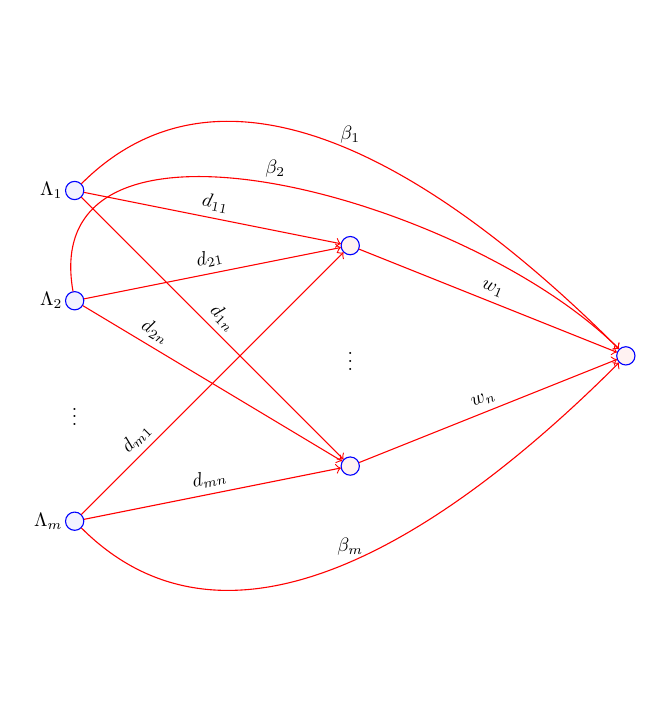
\begin{tikzpicture}[scale=0.7, every node/.style={scale=0.7}]
        \node (S1) at (0,0) [circle, draw=blue, fill=blue!5] {} node[left=.1cm] {$\Lambda_1$};
    \node (S2) at (0,-2) [circle, draw=blue, fill=blue!5] {} node at (S2)[left=.1cm] {$\Lambda_2$};
    \node (S3) at (0,-4)  {$\vdots$};
    \node (S4) at (0,-6) [circle, draw=blue, fill=blue!5] {} node at (S4) [left=.1cm] {$\Lambda_m$};

    \node (E) at (10,-3) [circle, draw=blue, fill=red!5] {};

    \node (F1) at (5,-1) [circle, draw=blue, fill=red!5] {};
    \node (F3) at (5,-3)  {$\vdots$};
    \node (F2) at (5,-5) [circle, draw=blue, fill=red!5] {};

    \draw [->, red] (F1) -- (E) node [midway, above, sloped, black] (TextNode) {$w_{1}$};
    \draw [->, red] (F2) -- (E) node [midway, above, sloped, black] (TextNode) {$w_{n}$};


    \draw [->, red] (S1) -- (F1) node [midway, above, sloped, black] (TextNode) {$d_{11}$};
    \draw [->, red] (S1) -- (F2) node [midway, above, sloped, black] (TextNode) {$d_{1n}$};
    \draw [->, red] (S2) -- (F1) node [midway, above, sloped, black] (TextNode) {$d_{21}$};
    \draw [->, red] (S2) -- (F2) node [near start, above, sloped, black] (TextNode) {$d_{2n}$};
    \draw [->, red] (S4) -- (F1) node [near start, above, sloped, black] (TextNode) {$d_{m1}$};
    \draw [->, red] (S4) -- (F2) node [midway, above, sloped, black] (TextNode) {$d_{mn}$};

    \draw [->, red] (S1) edge[out=45, in=135] node [above, black] {$\beta_1$} (E);
    \draw [->, red] (S4) edge[out=-45, in=-135] node [above, black] {$\beta_m$} (E);
    \draw [->, red] (S2) edge[out=100, in=135] node [above, black] {$\beta_2$} (E);

    \end{tikzpicture}
    \end{center}
}

%\frame{
%
%    \begin{center}
%    \begin{tikzpicture}
%
%    \draw [->] (0,0) -- (10,0);
%    \draw [->] (0,0) -- (0,8);
%    \node at (10,0) [below] {$\Lambda$};
%    \node at (0,8) [left] {PoA};
%
%    %\node (social) at (3,0) [below] {$x^*$};
%    %\node (selfish) at (7,0) [below] {$\tilde x$};
%
%    \draw [dashed] (3,0) -- (3,8);
%    \draw [dashed] (7,0) -- (7,8);
%
%    \draw [thick] (0,3) -- (3,3);
%    \draw (3,3) edge[thick,out=0,in=-100] (7,6);
%    \draw (7,6) edge[thick,out=-80,in=170] (10,4);
%
%    \node at (1.5,4) [text width=2cm]{Low level of demand};
%    \node at (5,6) {Inefficient system};
%    \node at (8.5,2) [text width=2cm]{High level of demand};
%
%    \end{tikzpicture}
%
%    \end{center}
%}

\frame{
    \begin{center}
    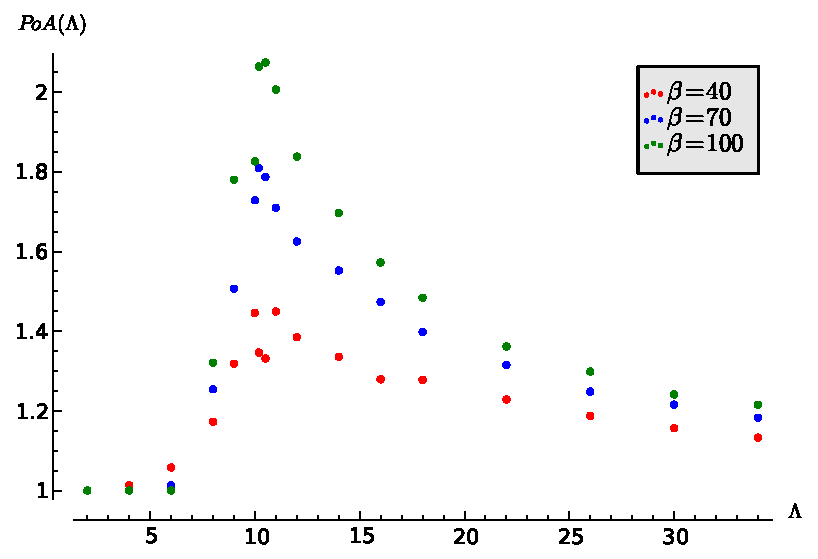
\includegraphics[width=.8\textwidth]{./Images/varyinglambda.pdf}
    \end{center}
}

\frame{
        \textbf{Price of Anarchy in Public Services} \textit{EJORS}, 2013.
}


\frame{
    \begin{center}
    \Huge What about the controllers?
    \end{center}
}

\frame{
    \begin{center}
    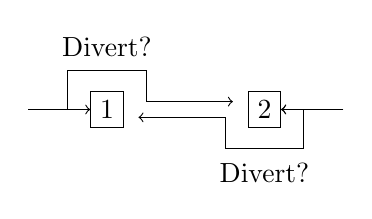
\begin{tikzpicture}
    \node (A) at (0,0) [draw] {1};
    \node (B) at (2,0) [draw] {2};
    \draw [->] (-1,0) -- (A);
    \draw [->] (3,0) -- (B);
    \draw [->] (-1,0) -- ($(A)+(-.5,0)$) -- ($(A)+(-.5,.5)$) -- ($(A)+(.5,.5)$) -- ($(A)+(.5,.1)$) -- ($(B)+(-.4,.1)$);
    \draw [->] (3,0) -- ($(B)+(.5,0)$) -- ($(B)+(.5,-.5)$) -- ($(B)+(-.5,-.5)$) -- ($(B)+(-.5,-.1)$) -- ($(A)+(.4,-.1)$);
    \draw [->] (3,0) -- (B);
    \node at ($(A) + (0,.8)$) {Divert?};
    \node at ($(B) + (0,-.8)$) {Divert?};
    \end{tikzpicture}
    \end{center}
}

%\frame{
%    \begin{center}
%    \begin{tikzpicture}
%    \draw  (0,0) rectangle (4,3);
%    \draw [dashed, red, thick] (0,1) -- (4,1);
%    \draw [dashed, red, thick] (3,0) -- (3,3);
%    \node at (-.5,1) {$K_{1}$};
%    \node at (3,3.25) {$K_{2}$};
%    \node at (1.5,2) {$\lambda_{h}^{(a)}$};
%    \node at (3.5,2) {$\lambda_{h}^{(b)}$};
%    \node at (1.5,.5) {$\lambda_{h}^{(c)}$};
%    \node at (3.5,.5) {$\lambda_{h}^{(d)}$};
%    \end{tikzpicture}
%    \end{center}
%}
%
%\frame{
%    \begin{center}
%    \begin{tabular}{cl}
%    \toprule
%        Parameter                   & Interpretation\\
%        \midrule
%        $h\in\{1,2\}$               & CCU\\
%        $c_h$                       & Capacity of CCU\\
%        $K_h$                       & Cutoff strategy of CCU\\
%        $\lambda_{h}^{\text{area}}$ & Demand rate\\
%        $\mu_{h}$                   & Service rate of CCU\\
%        \toprule
%        \end{tabular}
%    \end{center}
%}
%
%\frame{
%\begin{center}
%    \only<1>{
%        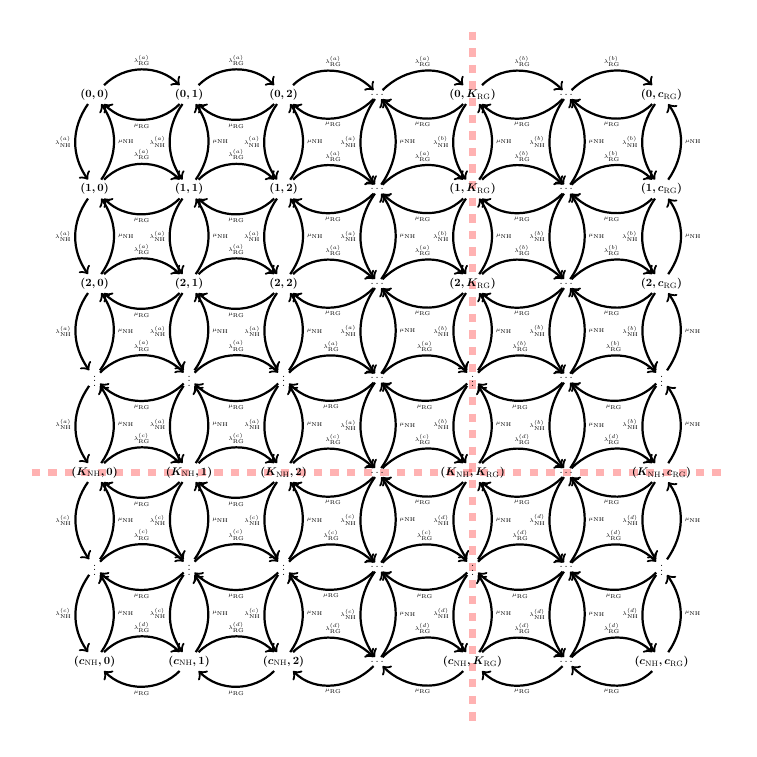
\begin{tikzpicture}[scale=.4, every node/.style={scale=0.4}]
    % -----------------------------------------------
    % Boundaries ------------------------------------
    % -----------------------------------------------
    \draw [dashed, line width=1mm, red, opacity=.3] (12,2) -- (12,-20);
    \draw [dashed, line width=1mm, red, opacity=.3] (-2,-12) -- (20,-12);
    %\tikzstyle{state}=[ellipse, draw, fill=blue!10, minimum width=2cm];
    %\tikzstyle{state}=[rectangle, draw, fill=blue!10, minimum width=2cm];
    \tikzstyle{state}=[minimum width=2cm, font=\boldmath];
    %\draw  (0,0) rectangle (4,3);
    %\draw [dashed, red, thick] (0,1) -- (4,1);
    %\draw [dashed, red, thick] (3,0) -- (3,3);
    % -----------------------------------------------
    % First row--------------------------------------
    % -----------------------------------------------
    \node (aa) [state] at (0,0) {$(0,0)$};
    \node (ab) [state] at ($(aa) + (3,0)$) {$(0,1)$};
    \node (ac) [state] at ($(ab) + (3,0)$) {$(0,2)$};
    \node (ellipsisa1) at ($(ac) + (3,0)$) {$\dots$};
    \node(ak) [state] at ($(ellipsisa1) + (3,0)$) {$(0,K_{\RG})$};
    \node (ellipsisa2) at ($(ak) + (3,0)$) {$\dots$};
    \node(az) [state] at ($(ellipsisa2) + (3,0)$) {$(0,c_{\RG})$};
    % Transitions -----------------------------------
    % On Row:
    \draw (aa) edge[out=45,in=135,->,thick] node [above] {\tiny$\lambda_{\RG}^{(a)}$} (ab);
    \draw (aa) edge[out=-45,in=-135,<-,thick] node [below] {\tiny$\mu_{\RG}$} (ab);

    \draw (ab) edge[out=45,in=135,->,thick] node [above] {\tiny$\lambda_{\RG}^{(a)}$} (ac);
    \draw (ab) edge[out=-45,in=-135,<-,thick] node [below] {\tiny$\mu_{\RG}$} (ac);

    \draw (ac) edge[out=45,in=135,->,thick] node [above] {\tiny$\lambda_{\RG}^{(a)}$} (ellipsisa1);
    \draw (ac) edge[out=-45,in=-135,<-,thick] node [below] {\tiny$\mu_{\RG}$} (ellipsisa1);

    \draw (ellipsisa1) edge[out=45,in=135,->,thick] node [above] {\tiny$\lambda_{\RG}^{(a)}$} (ak);
    \draw (ellipsisa1) edge[out=-45,in=-135,<-,thick] node [below] {\tiny$\mu_{\RG}$} (ak);

    \draw (ak) edge[out=45,in=135,->,thick] node [above] {\tiny$\lambda_{\RG}^{(b)}$} (ellipsisa2);
    \draw (ak) edge[out=-45,in=-135,<-,thick] node [below] {\tiny$\mu_{\RG}$} (ellipsisa2);

    \draw (ellipsisa2) edge[out=45,in=135,->,thick] node [above] {\tiny$\lambda_{\RG}^{(b)}$} (az);
    \draw (ellipsisa2) edge[out=-45,in=-135,<-,thick] node [below] {\tiny$\mu_{\RG}$} (az);
    % -----------------------------------------------
    % Second row--------------------------------------
    % -----------------------------------------------
    \node (ba) [state] at (0,-3) {$(1,0)$};
    \node (bb) [state] at ($(ba) + (3,0)$) {$(1,1)$};
    \node (bc) [state] at ($(bb) + (3,0)$) {$(1,2)$};
    \node (ellipsisb1) at ($(bc) + (3,0)$) {$\dots$};
    \node(bk) [state] at ($(ellipsisb1) + (3,0)$) {$(1,K_{\RG})$};
    \node (ellipsisb2) at ($(bk) + (3,0)$) {$\dots$};
    \node(bz) [state] at ($(ellipsisb2) + (3,0)$) {$(1,c_{\RG})$};
    % Transitions -----------------------------------
    % On Row:
    \draw (ba) edge[out=45,in=135,->,thick] node [above] {\tiny$\lambda_{\RG}^{(a)}$} (bb);
    \draw (ba) edge[out=-45,in=-135,<-,thick] node [below] {\tiny$\mu_{\RG}$} (bb);

    \draw (bb) edge[out=45,in=135,->,thick] node [above] {\tiny$\lambda_{\RG}^{(a)}$} (bc);
    \draw (bb) edge[out=-45,in=-135,<-,thick] node [below] {\tiny$\mu_{\RG}$} (bc);

    \draw (bc) edge[out=45,in=135,->,thick] node [above] {\tiny$\lambda_{\RG}^{(a)}$} (ellipsisb1);
    \draw (bc) edge[out=-45,in=-135,<-,thick] node [below] {\tiny$\mu_{\RG}$} (ellipsisb1);

    \draw (ellipsisb1) edge[out=45,in=135,->,thick] node [above] {\tiny$\lambda_{\RG}^{(a)}$} (bk);
    \draw (ellipsisb1) edge[out=-45,in=-135,<-,thick] node [below] {\tiny$\mu_{\RG}$} (bk);

    \draw (bk) edge[out=45,in=135,->,thick] node [above] {\tiny$\lambda_{\RG}^{(b)}$} (ellipsisb2);
    \draw (bk) edge[out=-45,in=-135,<-,thick] node [below] {\tiny$\mu_{\RG}$} (ellipsisb2);

    \draw (ellipsisb2) edge[out=45,in=135,->,thick] node [above] {\tiny$\lambda_{\RG}^{(b)}$} (bz);
    \draw (ellipsisb2) edge[out=-45,in=-135,<-,thick] node [below] {\tiny$\mu_{\RG}$} (bz);
    % With previous row:
    \draw (aa) edge[out=-125,in=125,->,thick] node [left] {\tiny$\lambda_{\NH}^{(a)}$} (ba);
    \draw (aa) edge[out=-55,in=55,<-,thick] node [right] {\tiny$\mu_{\NH}$} (ba);

    \draw (ab) edge[out=-125,in=125,->,thick] node [left] {\tiny$\lambda_{\NH}^{(a)}$} (bb);
    \draw (ab) edge[out=-55,in=55,<-,thick] node [right] {\tiny$\mu_{\NH}$} (bb);

    \draw (ac) edge[out=-125,in=125,->,thick] node [left] {\tiny$\lambda_{\NH}^{(a)}$} (bc);
    \draw (ac) edge[out=-55,in=55,<-,thick] node [right] {\tiny$\mu_{\NH}$} (bc);

    \draw (ellipsisa1) edge[out=-125,in=125,->,thick] node [left] {\tiny$\lambda_{\NH}^{(a)}$} (ellipsisb1);
    \draw (ellipsisa1) edge[out=-55,in=55,<-,thick] node [right] {\tiny$\mu_{\NH}$} (ellipsisb1);

    \draw (ak) edge[out=-125,in=125,->,thick] node [left] {\tiny$\lambda_{\NH}^{(b)}$} (bk);
    \draw (ak) edge[out=-55,in=55,<-,thick] node [right] {\tiny$\mu_{\NH}$} (bk);

    \draw (ellipsisa2) edge[out=-125,in=125,->,thick] node [left] {\tiny$\lambda_{\NH}^{(b)}$} (ellipsisb2);
    \draw (ellipsisa2) edge[out=-55,in=55,<-,thick] node [right] {\tiny$\mu_{\NH}$} (ellipsisb2);

    \draw (az) edge[out=-125,in=125,->,thick] node [left] {\tiny$\lambda_{\NH}^{(b)}$} (bz);
    \draw (az) edge[out=-55,in=55,<-,thick] node [right] {\tiny$\mu_{\NH}$} (bz);
    % -----------------------------------------------
    % Third row--------------------------------------
    % -----------------------------------------------
    \node (ca) [state] at (0,-6) {$(2,0)$};
    \node (cb) [state] at ($(ca) + (3,0)$) {$(2,1)$};
    \node (cc) [state] at ($(cb) + (3,0)$) {$(2,2)$};
    \node (ellipsisc1) at ($(cc) + (3,0)$) {$\dots$};
    \node(ck) [state] at ($(ellipsisc1) + (3,0)$) {$(2,K_{\RG})$};
    \node (ellipsisc2) at ($(ck) + (3,0)$) {$\dots$};
    \node(cz) [state] at ($(ellipsisc2) + (3,0)$) {$(2,c_{\RG})$};
    % Transitions -----------------------------------
    % On Row:
    \draw (ca) edge[out=45,in=135,->,thick] node [above] {\tiny$\lambda_{\RG}^{(a)}$} (cb);
    \draw (ca) edge[out=-45,in=-135,<-,thick] node [below] {\tiny$\mu_{\RG}$} (cb);

    \draw (cb) edge[out=45,in=135,->,thick] node [above] {\tiny$\lambda_{\RG}^{(a)}$} (cc);
    \draw (cb) edge[out=-45,in=-135,<-,thick] node [below] {\tiny$\mu_{\RG}$} (cc);

    \draw (cc) edge[out=45,in=135,->,thick] node [above] {\tiny$\lambda_{\RG}^{(a)}$} (ellipsisc1);
    \draw (cc) edge[out=-45,in=-135,<-,thick] node [below] {\tiny$\mu_{\RG}$} (ellipsisc1);

    \draw (ellipsisc1) edge[out=45,in=135,->,thick] node [above] {\tiny$\lambda_{\RG}^{(a)}$} (ck);
    \draw (ellipsisc1) edge[out=-45,in=-135,<-,thick] node [below] {\tiny$\mu_{\RG}$} (ck);

    \draw (ck) edge[out=45,in=135,->,thick] node [above] {\tiny$\lambda_{\RG}^{(b)}$} (ellipsisc2);
    \draw (ck) edge[out=-45,in=-135,<-,thick] node [below] {\tiny$\mu_{\RG}$} (ellipsisc2);

    \draw (ellipsisc2) edge[out=45,in=135,->,thick] node [above] {\tiny$\lambda_{\RG}^{(b)}$} (cz);
    \draw (ellipsisc2) edge[out=-45,in=-135,<-,thick] node [below] {\tiny$\mu_{\RG}$} (cz);
    % With previous row:
    \draw (ba) edge[out=-125,in=125,->,thick] node [left] {\tiny$\lambda_{\NH}^{(a)}$} (ca);
    \draw (ba) edge[out=-55,in=55,<-,thick] node [right] {\tiny$\mu_{\NH}$} (ca);

    \draw (bb) edge[out=-125,in=125,->,thick] node [left] {\tiny$\lambda_{\NH}^{(a)}$} (cb);
    \draw (bb) edge[out=-55,in=55,<-,thick] node [right] {\tiny$\mu_{\NH}$} (cb);

    \draw (bc) edge[out=-125,in=125,->,thick] node [left] {\tiny$\lambda_{\NH}^{(a)}$} (cc);
    \draw (bc) edge[out=-55,in=55,<-,thick] node [right] {\tiny$\mu_{\NH}$} (cc);

    \draw (ellipsisb1) edge[out=-125,in=125,->,thick] node [left] {\tiny$\lambda_{\NH}^{(a)}$} (ellipsisc1);
    \draw (ellipsisb1) edge[out=-55,in=55,<-,thick] node [right] {\tiny$\mu_{\NH}$} (ellipsisc1);

    \draw (bk) edge[out=-125,in=125,->,thick] node [left] {\tiny$\lambda_{\NH}^{(b)}$} (ck);
    \draw (bk) edge[out=-55,in=55,<-,thick] node [right] {\tiny$\mu_{\NH}$} (ck);

    \draw (ellipsisb2) edge[out=-125,in=125,->,thick] node [left] {\tiny$\lambda_{\NH}^{(b)}$} (ellipsisc2);
    \draw (ellipsisb2) edge[out=-55,in=55,<-,thick] node [right] {\tiny$\mu_{\NH}$} (ellipsisc2);

    \draw (bz) edge[out=-125,in=125,->,thick] node [left] {\tiny$\lambda_{\NH}^{(b)}$} (cz);
    \draw (bz) edge[out=-55,in=55,<-,thick] node [right] {\tiny$\mu_{\NH}$} (cz);
    % -----------------------------------------------
    % Fourth row--------------------------------------
    % -----------------------------------------------
    \node (da) at (0,-9) {$\vdots$};
    \node (db) at ($(da) + (3,0)$) {$\vdots$};
    \node (dc) at ($(db) + (3,0)$) {$\vdots$};
    \node (ellipsisd1) at ($(dc) + (3,0)$) {$\dots$};
    \node(dk) at ($(ellipsisd1) + (3,0)$) {$\vdots$};
    \node (ellipsisd2) at ($(dk) + (3,0)$) {$\dots$};
    \node(dz) at ($(ellipsisd2) + (3,0)$) {$\vdots$};
    % Transitions -----------------------------------
    % On Row:
    \draw (da) edge[out=45,in=135,->,thick] node [above] {\tiny$\lambda_{\RG}^{(a)}$} (db);
    \draw (da) edge[out=-45,in=-135,<-,thick] node [below] {\tiny$\mu_{\RG}$} (db);

    \draw (db) edge[out=45,in=135,->,thick] node [above] {\tiny$\lambda_{\RG}^{(a)}$} (dc);
    \draw (db) edge[out=-45,in=-135,<-,thick] node [below] {\tiny$\mu_{\RG}$} (dc);

    \draw (dc) edge[out=45,in=135,->,thick] node [above] {\tiny$\lambda_{\RG}^{(a)}$} (ellipsisd1);
    \draw (dc) edge[out=-45,in=-135,<-,thick] node [below] {\tiny$\mu_{\RG}$} (ellipsisd1);

    \draw (ellipsisd1) edge[out=45,in=135,->,thick] node [above] {\tiny$\lambda_{\RG}^{(a)}$} (dk);
    \draw (ellipsisd1) edge[out=-45,in=-135,<-,thick] node [below] {\tiny$\mu_{\RG}$} (dk);

    \draw (dk) edge[out=45,in=135,->,thick] node [above] {\tiny$\lambda_{\RG}^{(b)}$} (ellipsisd2);
    \draw (dk) edge[out=-45,in=-135,<-,thick] node [below] {\tiny$\mu_{\RG}$} (ellipsisd2);

    \draw (ellipsisd2) edge[out=45,in=135,->,thick] node [above] {\tiny$\lambda_{\RG}^{(b)}$} (dz);
    \draw (ellipsisd2) edge[out=-45,in=-135,<-,thick] node [below] {\tiny$\mu_{\RG}$} (dz);
    % With previous row:
    \draw (ca) edge[out=-125,in=125,->,thick] node [left] {\tiny$\lambda_{\NH}^{(a)}$} (da);
    \draw (ca) edge[out=-55,in=55,<-,thick] node [right] {\tiny$\mu_{\NH}$} (da);

    \draw (cb) edge[out=-125,in=125,->,thick] node [left] {\tiny$\lambda_{\NH}^{(a)}$} (db);
    \draw (cb) edge[out=-55,in=55,<-,thick] node [right] {\tiny$\mu_{\NH}$} (db);

    \draw (cc) edge[out=-125,in=125,->,thick] node [left] {\tiny$\lambda_{\NH}^{(a)}$} (dc);
    \draw (cc) edge[out=-55,in=55,<-,thick] node [right] {\tiny$\mu_{\NH}$} (dc);

    \draw (ellipsisc1) edge[out=-125,in=125,->,thick] node [left] {\tiny$\lambda_{\NH}^{(a)}$} (ellipsisd1);
    \draw (ellipsisc1) edge[out=-55,in=55,<-,thick] node [right] {\tiny$\mu_{\NH}$} (ellipsisd1);

    \draw (ck) edge[out=-125,in=125,->,thick] node [left] {\tiny$\lambda_{\NH}^{(b)}$} (dk);
    \draw (ck) edge[out=-55,in=55,<-,thick] node [right] {\tiny$\mu_{\NH}$} (dk);

    \draw (ellipsisc2) edge[out=-125,in=125,->,thick] node [left] {\tiny$\lambda_{\NH}^{(b)}$} (ellipsisd2);
    \draw (ellipsisc2) edge[out=-55,in=55,<-,thick] node [right] {\tiny$\mu_{\NH}$} (ellipsisd2);

    \draw (cz) edge[out=-125,in=125,->,thick] node [left] {\tiny$\lambda_{\NH}^{(b)}$} (dz);
    \draw (cz) edge[out=-55,in=55,<-,thick] node [right] {\tiny$\mu_{\NH}$} (dz);
    % -----------------------------------------------
    % Fifth row--------------------------------------
    % -----------------------------------------------
    \node (ea) [state] at (0,-12) {$(K_{\NH},0)$};
    \node (eb) [state] at ($(ea) + (3,0)$) {$(K_{\NH},1)$};
    \node (ec) [state] at ($(eb) + (3,0)$) {$(K_{\NH},2)$};
    \node (ellipsise1) at ($(ec) + (3,0)$) {$\dots$};
    \node(ek) [state] at ($(ellipsise1) + (3,0)$) {$(K_{\NH},K_{\RG})$};
    \node (ellipsise2) at ($(ek) + (3,0)$) {$\dots$};
    \node(ez) [state] at ($(ellipsise2) + (3,0)$) {$(K_{\NH},c_{\RG})$};
    % Transitions -----------------------------------
    % On Row:
    \draw (ea) edge[out=45,in=135,->,thick] node [above] {\tiny$\lambda_{\RG}^{(c)}$} (eb);
    \draw (ea) edge[out=-45,in=-135,<-,thick] node [below] {\tiny$\mu_{\RG}$} (eb);

    \draw (eb) edge[out=45,in=135,->,thick] node [above] {\tiny$\lambda_{\RG}^{(c)}$} (ec);
    \draw (eb) edge[out=-45,in=-135,<-,thick] node [below] {\tiny$\mu_{\RG}$} (ec);

    \draw (ec) edge[out=45,in=135,->,thick] node [above] {\tiny$\lambda_{\RG}^{(c)}$} (ellipsise1);
    \draw (ec) edge[out=-45,in=-135,<-,thick] node [below] {\tiny$\mu_{\RG}$} (ellipsise1);

    \draw (ellipsise1) edge[out=45,in=135,->,thick] node [above] {\tiny$\lambda_{\RG}^{(c)}$} (ek);
    \draw (ellipsise1) edge[out=-45,in=-135,<-,thick] node [below] {\tiny$\mu_{\RG}$} (ek);

    \draw (ek) edge[out=45,in=135,->,thick] node [above] {\tiny$\lambda_{\RG}^{(d)}$} (ellipsise2);
    \draw (ek) edge[out=-45,in=-135,<-,thick] node [below] {\tiny$\mu_{\RG}$} (ellipsise2);

    \draw (ellipsise2) edge[out=45,in=135,->,thick] node [above] {\tiny$\lambda_{\RG}^{(d)}$} (ez);
    \draw (ellipsise2) edge[out=-45,in=-135,<-,thick] node [below] {\tiny$\mu_{\RG}$} (ez);
    % With previous row:
    \draw (da) edge[out=-125,in=125,->,thick] node [left] {\tiny$\lambda_{\NH}^{(a)}$} (ea);
    \draw (da) edge[out=-55,in=55,<-,thick] node [right] {\tiny$\mu_{\NH}$} (ea);

    \draw (db) edge[out=-125,in=125,->,thick] node [left] {\tiny$\lambda_{\NH}^{(a)}$} (eb);
    \draw (db) edge[out=-55,in=55,<-,thick] node [right] {\tiny$\mu_{\NH}$} (eb);

    \draw (dc) edge[out=-125,in=125,->,thick] node [left] {\tiny$\lambda_{\NH}^{(a)}$} (ec);
    \draw (dc) edge[out=-55,in=55,<-,thick] node [right] {\tiny$\mu_{\NH}$} (ec);

    \draw (ellipsisd1) edge[out=-125,in=125,->,thick] node [left] {\tiny$\lambda_{\NH}^{(a)}$} (ellipsise1);
    \draw (ellipsisd1) edge[out=-55,in=55,<-,thick] node [right] {\tiny$\mu_{\NH}$} (ellipsise1);

    \draw (dk) edge[out=-125,in=125,->,thick] node [left] {\tiny$\lambda_{\NH}^{(b)}$} (ek);
    \draw (dk) edge[out=-55,in=55,<-,thick] node [right] {\tiny$\mu_{\NH}$} (ek);

    \draw (ellipsisd2) edge[out=-125,in=125,->,thick] node [left] {\tiny$\lambda_{\NH}^{(b)}$} (ellipsise2);
    \draw (ellipsisd2) edge[out=-55,in=55,<-,thick] node [right] {\tiny$\mu_{\NH}$} (ellipsise2);

    \draw (dz) edge[out=-125,in=125,->,thick] node [left] {\tiny$\lambda_{\NH}^{(b)}$} (ez);
    \draw (dz) edge[out=-55,in=55,<-,thick] node [right] {\tiny$\mu_{\NH}$} (ez);
    % Sixth row--------------------------------------
    \node (fa) at (0,-15) {$\vdots$};
    \node (fb) at ($(fa) + (3,0)$) {$\vdots$};
    \node (fc) at ($(fb) + (3,0)$) {$\vdots$};
    \node (ellipsisf1) at ($(fc) + (3,0)$) {$\dots$};
    \node(fk) at ($(ellipsisf1) + (3,0)$) {$\vdots$};
    \node (ellipsisf2) at ($(fk) + (3,0)$) {$\dots$};
    \node(fz) at ($(ellipsisf2) + (3,0)$) {$\vdots$};
    % Transitions -----------------------------------
    % On Row:
    \draw (fa) edge[out=45,in=135,->,thick] node [above] {\tiny$\lambda_{\RG}^{(c)}$} (fb);
    \draw (fa) edge[out=-45,in=-135,<-,thick] node [below] {\tiny$\mu_{\RG}$} (fb);

    \draw (fb) edge[out=45,in=135,->,thick] node [above] {\tiny$\lambda_{\RG}^{(c)}$} (fc);
    \draw (fb) edge[out=-45,in=-135,<-,thick] node [below] {\tiny$\mu_{\RG}$} (fc);

    \draw (fc) edge[out=45,in=135,->,thick] node [above] {\tiny$\lambda_{\RG}^{(c)}$} (ellipsisf1);
    \draw (fc) edge[out=-45,in=-135,<-,thick] node [below] {\tiny$\mu_{\RG}$} (ellipsisf1);

    \draw (ellipsisf1) edge[out=45,in=135,->,thick] node [above] {\tiny$\lambda_{\RG}^{(c)}$} (fk);
    \draw (ellipsisf1) edge[out=-45,in=-135,<-,thick] node [below] {\tiny$\mu_{\RG}$} (fk);

    \draw (fk) edge[out=45,in=135,->,thick] node [above] {\tiny$\lambda_{\RG}^{(d)}$} (ellipsisf2);
    \draw (fk) edge[out=-45,in=-135,<-,thick] node [below] {\tiny$\mu_{\RG}$} (ellipsisf2);

    \draw (ellipsisf2) edge[out=45,in=135,->,thick] node [above] {\tiny$\lambda_{\RG}^{(d)}$} (fz);
    \draw (ellipsisf2) edge[out=-45,in=-135,<-,thick] node [below] {\tiny$\mu_{\RG}$} (fz);
    % With previous row:
    \draw (ea) edge[out=-125,in=125,->,thick] node [left] {\tiny$\lambda_{\NH}^{(c)}$} (fa);
    \draw (ea) edge[out=-55,in=55,<-,thick] node [right] {\tiny$\mu_{\NH}$} (fa);

    \draw (eb) edge[out=-125,in=125,->,thick] node [left] {\tiny$\lambda_{\NH}^{(c)}$} (fb);
    \draw (eb) edge[out=-55,in=55,<-,thick] node [right] {\tiny$\mu_{\NH}$} (fb);

    \draw (ec) edge[out=-125,in=125,->,thick] node [left] {\tiny$\lambda_{\NH}^{(c)}$} (fc);
    \draw (ec) edge[out=-55,in=55,<-,thick] node [right] {\tiny$\mu_{\NH}$} (fc);

    \draw (ellipsise1) edge[out=-125,in=125,->,thick] node [left] {\tiny$\lambda_{\NH}^{(c)}$} (ellipsisf1);
    \draw (ellipsise1) edge[out=-55,in=55,<-,thick] node [right] {\tiny$\mu_{\NH}$} (ellipsisf1);

    \draw (ek) edge[out=-125,in=125,->,thick] node [left] {\tiny$\lambda_{\NH}^{(d)}$} (fk);
    \draw (ek) edge[out=-55,in=55,<-,thick] node [right] {\tiny$\mu_{\NH}$} (fk);

    \draw (ellipsise2) edge[out=-125,in=125,->,thick] node [left] {\tiny$\lambda_{\NH}^{(d)}$} (ellipsisf2);
    \draw (ellipsise2) edge[out=-55,in=55,<-,thick] node [right] {\tiny$\mu_{\NH}$} (ellipsisf2);

    \draw (ez) edge[out=-125,in=125,->,thick] node [left] {\tiny$\lambda_{\NH}^{(d)}$} (fz);
    \draw (ez) edge[out=-55,in=55,<-,thick] node [right] {\tiny$\mu_{\NH}$} (fz);
    % Final row--------------------------------------
    \node (za) [state] at (0,-18) {$(c_{\NH},0)$};
    \node (zb) [state] at ($(za) + (3,0)$) {$(c_{\NH},1)$};
    \node (zc) [state] at ($(zb) + (3,0)$) {$(c_{\NH},2)$};
    \node (ellipsisz1) at ($(zc) + (3,0)$) {$\dots$};
    \node(zk) [state] at ($(ellipsisz1) + (3,0)$) {$(c_{\NH},K_{\RG})$};
    \node (ellipsisz2) at ($(zk) + (3,0)$) {$\dots$};
    \node(zz) [state] at ($(ellipsisz2) + (3,0)$) {$(c_{\NH},c_{\RG})$};
    % Transitions -----------------------------------
    % On Row:
    \draw (za) edge[out=45,in=135,->,thick] node [above] {\tiny$\lambda_{\RG}^{(d)}$} (zb);
    \draw (za) edge[out=-45,in=-135,<-,thick] node [below] {\tiny$\mu_{\RG}$} (zb);

    \draw (zb) edge[out=45,in=135,->,thick] node [above] {\tiny$\lambda_{\RG}^{(d)}$} (zc);
    \draw (zb) edge[out=-45,in=-135,<-,thick] node [below] {\tiny$\mu_{\RG}$} (zc);

    \draw (zc) edge[out=45,in=135,->,thick] node [above] {\tiny$\lambda_{\RG}^{(d)}$} (ellipsisz1);
    \draw (zc) edge[out=-45,in=-135,<-,thick] node [below] {\tiny$\mu_{\RG}$} (ellipsisz1);

    \draw (ellipsisz1) edge[out=45,in=135,->,thick] node [above] {\tiny$\lambda_{\RG}^{(d)}$} (zk);
    \draw (ellipsisz1) edge[out=-45,in=-135,<-,thick] node [below] {\tiny$\mu_{\RG}$} (zk);

    \draw (zk) edge[out=45,in=135,->,thick] node [above] {\tiny$\lambda_{\RG}^{(d)}$} (ellipsisz2);
    \draw (zk) edge[out=-45,in=-135,<-,thick] node [below] {\tiny$\mu_{\RG}$} (ellipsisz2);

    \draw (ellipsisz2) edge[out=45,in=135,->,thick] node [above] {\tiny$\lambda_{\RG}^{(d)}$} (zz);
    \draw (ellipsisz2) edge[out=-45,in=-135,<-,thick] node [below] {\tiny$\mu_{\RG}$} (zz);
    % With previous row:
    \draw (fa) edge[out=-125,in=125,->,thick] node [left] {\tiny$\lambda_{\NH}^{(c)}$} (za);
    \draw (fa) edge[out=-55,in=55,<-,thick] node [right] {\tiny$\mu_{\NH}$} (za);

    \draw (fb) edge[out=-125,in=125,->,thick] node [left] {\tiny$\lambda_{\NH}^{(c)}$} (zb);
    \draw (fb) edge[out=-55,in=55,<-,thick] node [right] {\tiny$\mu_{\NH}$} (zb);

    \draw (fc) edge[out=-125,in=125,->,thick] node [left] {\tiny$\lambda_{\NH}^{(c)}$} (zc);
    \draw (fc) edge[out=-55,in=55,<-,thick] node [right] {\tiny$\mu_{\NH}$} (zc);

    \draw (ellipsisf1) edge[out=-125,in=125,->,thick] node [left] {\tiny$\lambda_{\NH}^{(c)}$} (ellipsisz1);
    \draw (ellipsisf1) edge[out=-55,in=55,<-,thick] node [right] {\tiny$\mu_{\NH}$} (ellipsisz1);

    \draw (fk) edge[out=-125,in=125,->,thick] node [left] {\tiny$\lambda_{\NH}^{(d)}$} (zk);
    \draw (fk) edge[out=-55,in=55,<-,thick] node [right] {\tiny$\mu_{\NH}$} (zk);

    \draw (ellipsisf2) edge[out=-125,in=125,->,thick] node [left] {\tiny$\lambda_{\NH}^{(d)}$} (ellipsisz2);
    \draw (ellipsisf2) edge[out=-55,in=55,<-,thick] node [right] {\tiny$\mu_{\NH}$} (ellipsisz2);

    \draw (fz) edge[out=-125,in=125,->,thick] node [left] {\tiny$\lambda_{\NH}^{(d)}$} (zz);
    \draw (fz) edge[out=-55,in=55,<-,thick] node [right] {\tiny$\mu_{\NH}$} (zz);

\end{tikzpicture}

%    }
%    \only<2>{
%    \begin{tikzpicture}[scale=1, every node/.style={scale=1}]
%    % -----------------------------------------------
%    % Boundaries ------------------------------------
%    % -----------------------------------------------
%    \draw [dashed, line width=1mm, red, opacity=.3] (2,-3) -- (10,-3);
%    \draw [dashed, line width=1mm, red, opacity=.3] (6,1) -- (6,-7);
%    %\tikzstyle{state}=[ellipse, draw, fill=blue!10, minimum width=2cm];
%    %\tikzstyle{state}=[rectangle, draw, fill=blue!10, minimum width=2cm];
%    \tikzstyle{state}=[minimum width=2cm, font=\boldmath];
%
%    % -----------------------------------------------
%    % Fourth row--------------------------------------
%    % -----------------------------------------------
%    \node (ellipsisd1) at ($(0,0) + (3,0)$) {$\dots$};
%    \node(dk) at ($(ellipsisd1) + (3,0)$) {$\vdots$};
%    \node (ellipsisd2) at ($(dk) + (3,0)$) {$\dots$};
%    % Transitions -----------------------------------
%    % On Row:
%    \draw (ellipsisd1) edge[out=45,in=135,->,thick] node [above] {\tiny$\lambda_{\RG}^{(a)}$} (dk);
%    \draw (ellipsisd1) edge[out=-45,in=-135,<-,thick] node [below] {\tiny$\mu_{\RG}$} (dk);
%
%    \draw (dk) edge[out=45,in=135,->,thick] node [above] {\tiny$\lambda_{\RG}^{(b)}$} (ellipsisd2);
%    \draw (dk) edge[out=-45,in=-135,<-,thick] node [below] {\tiny$\mu_{\RG}$} (ellipsisd2);
%
%    % -----------------------------------------------
%    % Fifth row--------------------------------------
%    % -----------------------------------------------
%    \node (ellipsise1) at ($(0,-3) + (3,0)$) {$\dots$};
%    \node(ek) [state] at ($(ellipsise1) + (3,0)$) {$(K_{\NH},K_{\RG})$};
%    \node (ellipsise2) at ($(ek) + (3,0)$) {$\dots$};
%    % Transitions -----------------------------------
%    % On Row:
%    \draw (ellipsise1) edge[out=45,in=135,->,thick] node [above] {\tiny$\lambda_{\RG}^{(c)}$} (ek);
%    \draw (ellipsise1) edge[out=-45,in=-135,<-,thick] node [below] {\tiny$\mu_{\RG}$} (ek);
%
%    \draw (ek) edge[out=45,in=135,->,thick] node [above] {\tiny$\lambda_{\RG}^{(d)}$} (ellipsise2);
%    \draw (ek) edge[out=-45,in=-135,<-,thick] node [below] {\tiny$\mu_{\RG}$} (ellipsise2);
%
%    % With previous row:
%
%    \draw (ellipsisd1) edge[out=-125,in=125,->,thick] node [left] {\tiny$\lambda_{\NH}^{(a)}$} (ellipsise1);
%    \draw (ellipsisd1) edge[out=-55,in=55,<-,thick] node [right] {\tiny$\mu_{\NH}$} (ellipsise1);
%
%    \draw (dk) edge[out=-125,in=125,->,thick] node [left] {\tiny$\lambda_{\NH}^{(b)}$} (ek);
%    \draw (dk) edge[out=-55,in=55,<-,thick] node [right] {\tiny$\mu_{\NH}$} (ek);
%
%    \draw (ellipsisd2) edge[out=-125,in=125,->,thick] node [left] {\tiny$\lambda_{\NH}^{(b)}$} (ellipsise2);
%    \draw (ellipsisd2) edge[out=-55,in=55,<-,thick] node [right] {\tiny$\mu_{\NH}$} (ellipsise2);
%    % Sixth row--------------------------------------
%    \node (ellipsisf1) at ($(3,-3) + (0,-3)$) {$\dots$};
%    \node(fk) at ($(ellipsisf1) + (3,0)$) {$\vdots$};
%    \node (ellipsisf2) at ($(fk) + (3,0)$) {$\dots$};
%    % Transitions -----------------------------------
%    % On Row:
%
%    \draw (ellipsisf1) edge[out=45,in=135,->,thick] node [above] {\tiny$\lambda_{\RG}^{(c)}$} (fk);
%    \draw (ellipsisf1) edge[out=-45,in=-135,<-,thick] node [below] {\tiny$\mu_{\RG}$} (fk);
%
%    \draw (fk) edge[out=45,in=135,->,thick] node [above] {\tiny$\lambda_{\RG}^{(d)}$} (ellipsisf2);
%    \draw (fk) edge[out=-45,in=-135,<-,thick] node [below] {\tiny$\mu_{\RG}$} (ellipsisf2);
%
%    % With previous row:
%
%    \draw (ellipsise1) edge[out=-125,in=125,->,thick] node [left] {\tiny$\lambda_{\NH}^{(c)}$} (ellipsisf1);
%    \draw (ellipsise1) edge[out=-55,in=55,<-,thick] node [right] {\tiny$\mu_{\NH}$} (ellipsisf1);
%
%    \draw (ek) edge[out=-125,in=125,->,thick] node [left] {\tiny$\lambda_{\NH}^{(d)}$} (fk);
%    \draw (ek) edge[out=-55,in=55,<-,thick] node [right] {\tiny$\mu_{\NH}$} (fk);
%
%    \draw (ellipsise2) edge[out=-125,in=125,->,thick] node [left] {\tiny$\lambda_{\NH}^{(d)}$} (ellipsisf2);
%    \draw (ellipsise2) edge[out=-55,in=55,<-,thick] node [right] {\tiny$\mu_{\NH}$} (ellipsisf2);
%
%    \end{tikzpicture}
%    }
%\end{center}
%}
%
%\frame{
%\textbf{Theorem.}\\
%Let $f_{h}(k):[1,c_{\bar h}]\to[1,c_h]$ be the best response of player $h\in\{\NH, \RG\}$ to the diversion threshold of $\bar h\ne h$ ($\bar h\in\{\NH, \RG\}$).
%
%If $f_{h}(k)$ is a non-decreasing function in $k$ then the game has at least one Nash Equilibrium in Pure Strategies.\\
%}

%\frame{
%$$
%A =
%\begin{pmatrix}
%(U_{\NH}(1,1)-t)^2&\dots&(U_{\NH}(1,c_{\RG})-t)^2\\
%(U_{\NH}(2,1)-t)^2&\dots&(U_{\NH}(2,c_{\RG})-t)^2\\
%\vdots&\ddots&\vdots\\
%(U_{\NH}(c_{\NH},1)-t)^2&\dots&(U_{\NH}(c_{\NH},c_{\RG})-t)^2\\
%\end{pmatrix}
%$$
%\vspace{1cm}
%$$
%B =
%\begin{pmatrix}
%(U_{\RG}(1,1)-t)^2&\dots&(U_{\RG}(1,c_{\RG})-t)^2\\
%(U_{\RG}(2,1)-t)^2&\dots&(U_{\RG}(2,c_{\RG})-t)^2\\
%\vdots&\ddots&\vdots\\
%(U_{\RG}(c_{\RG},1)-t)^2&\dots&(U_{\RG}(c_{\RG},c_{\RG})-t)^2\\
%\end{pmatrix}
%$$
%}
%
%\frame{
%\begin{center}
%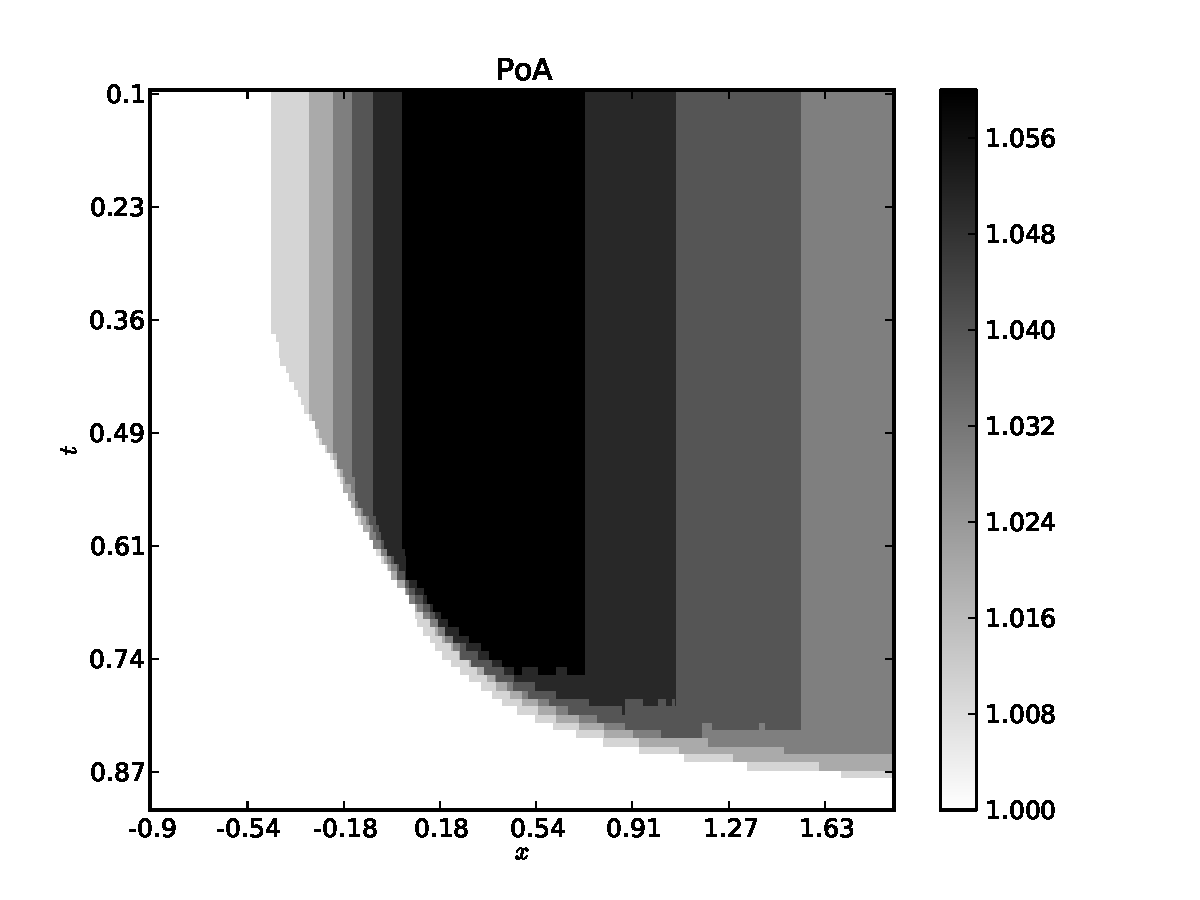
\includegraphics[width=.8\textwidth]{./Images/model2targetvdemand.pdf}
%\end{center}
%}

\frame{
\begin{center}
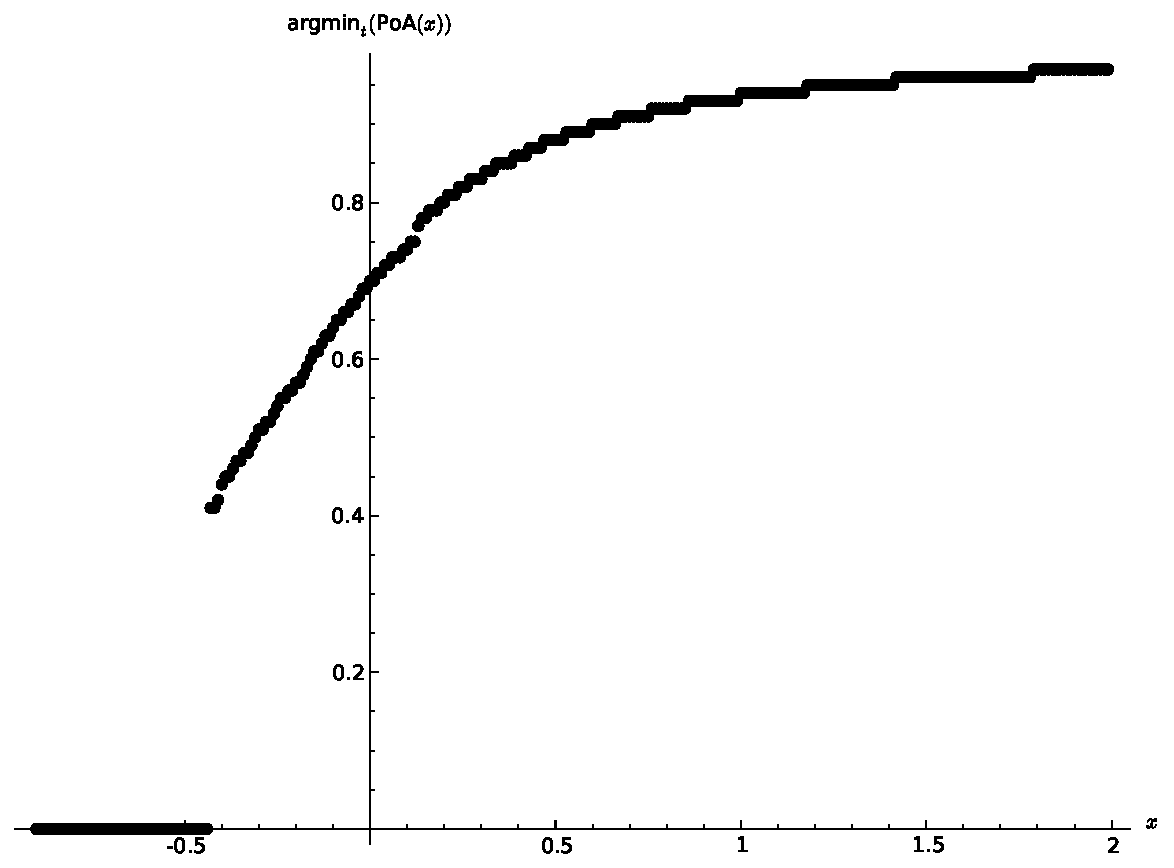
\includegraphics[width=.8\textwidth]{./Images/argminPoAmodel2.pdf}
\end{center}
}

\frame{
    \textbf{Measuring the Price of Anarchy in Critical Care Unit Interactions}, \textit{Submitted to OMEGA}

}

\frame{
    \begin{center}
        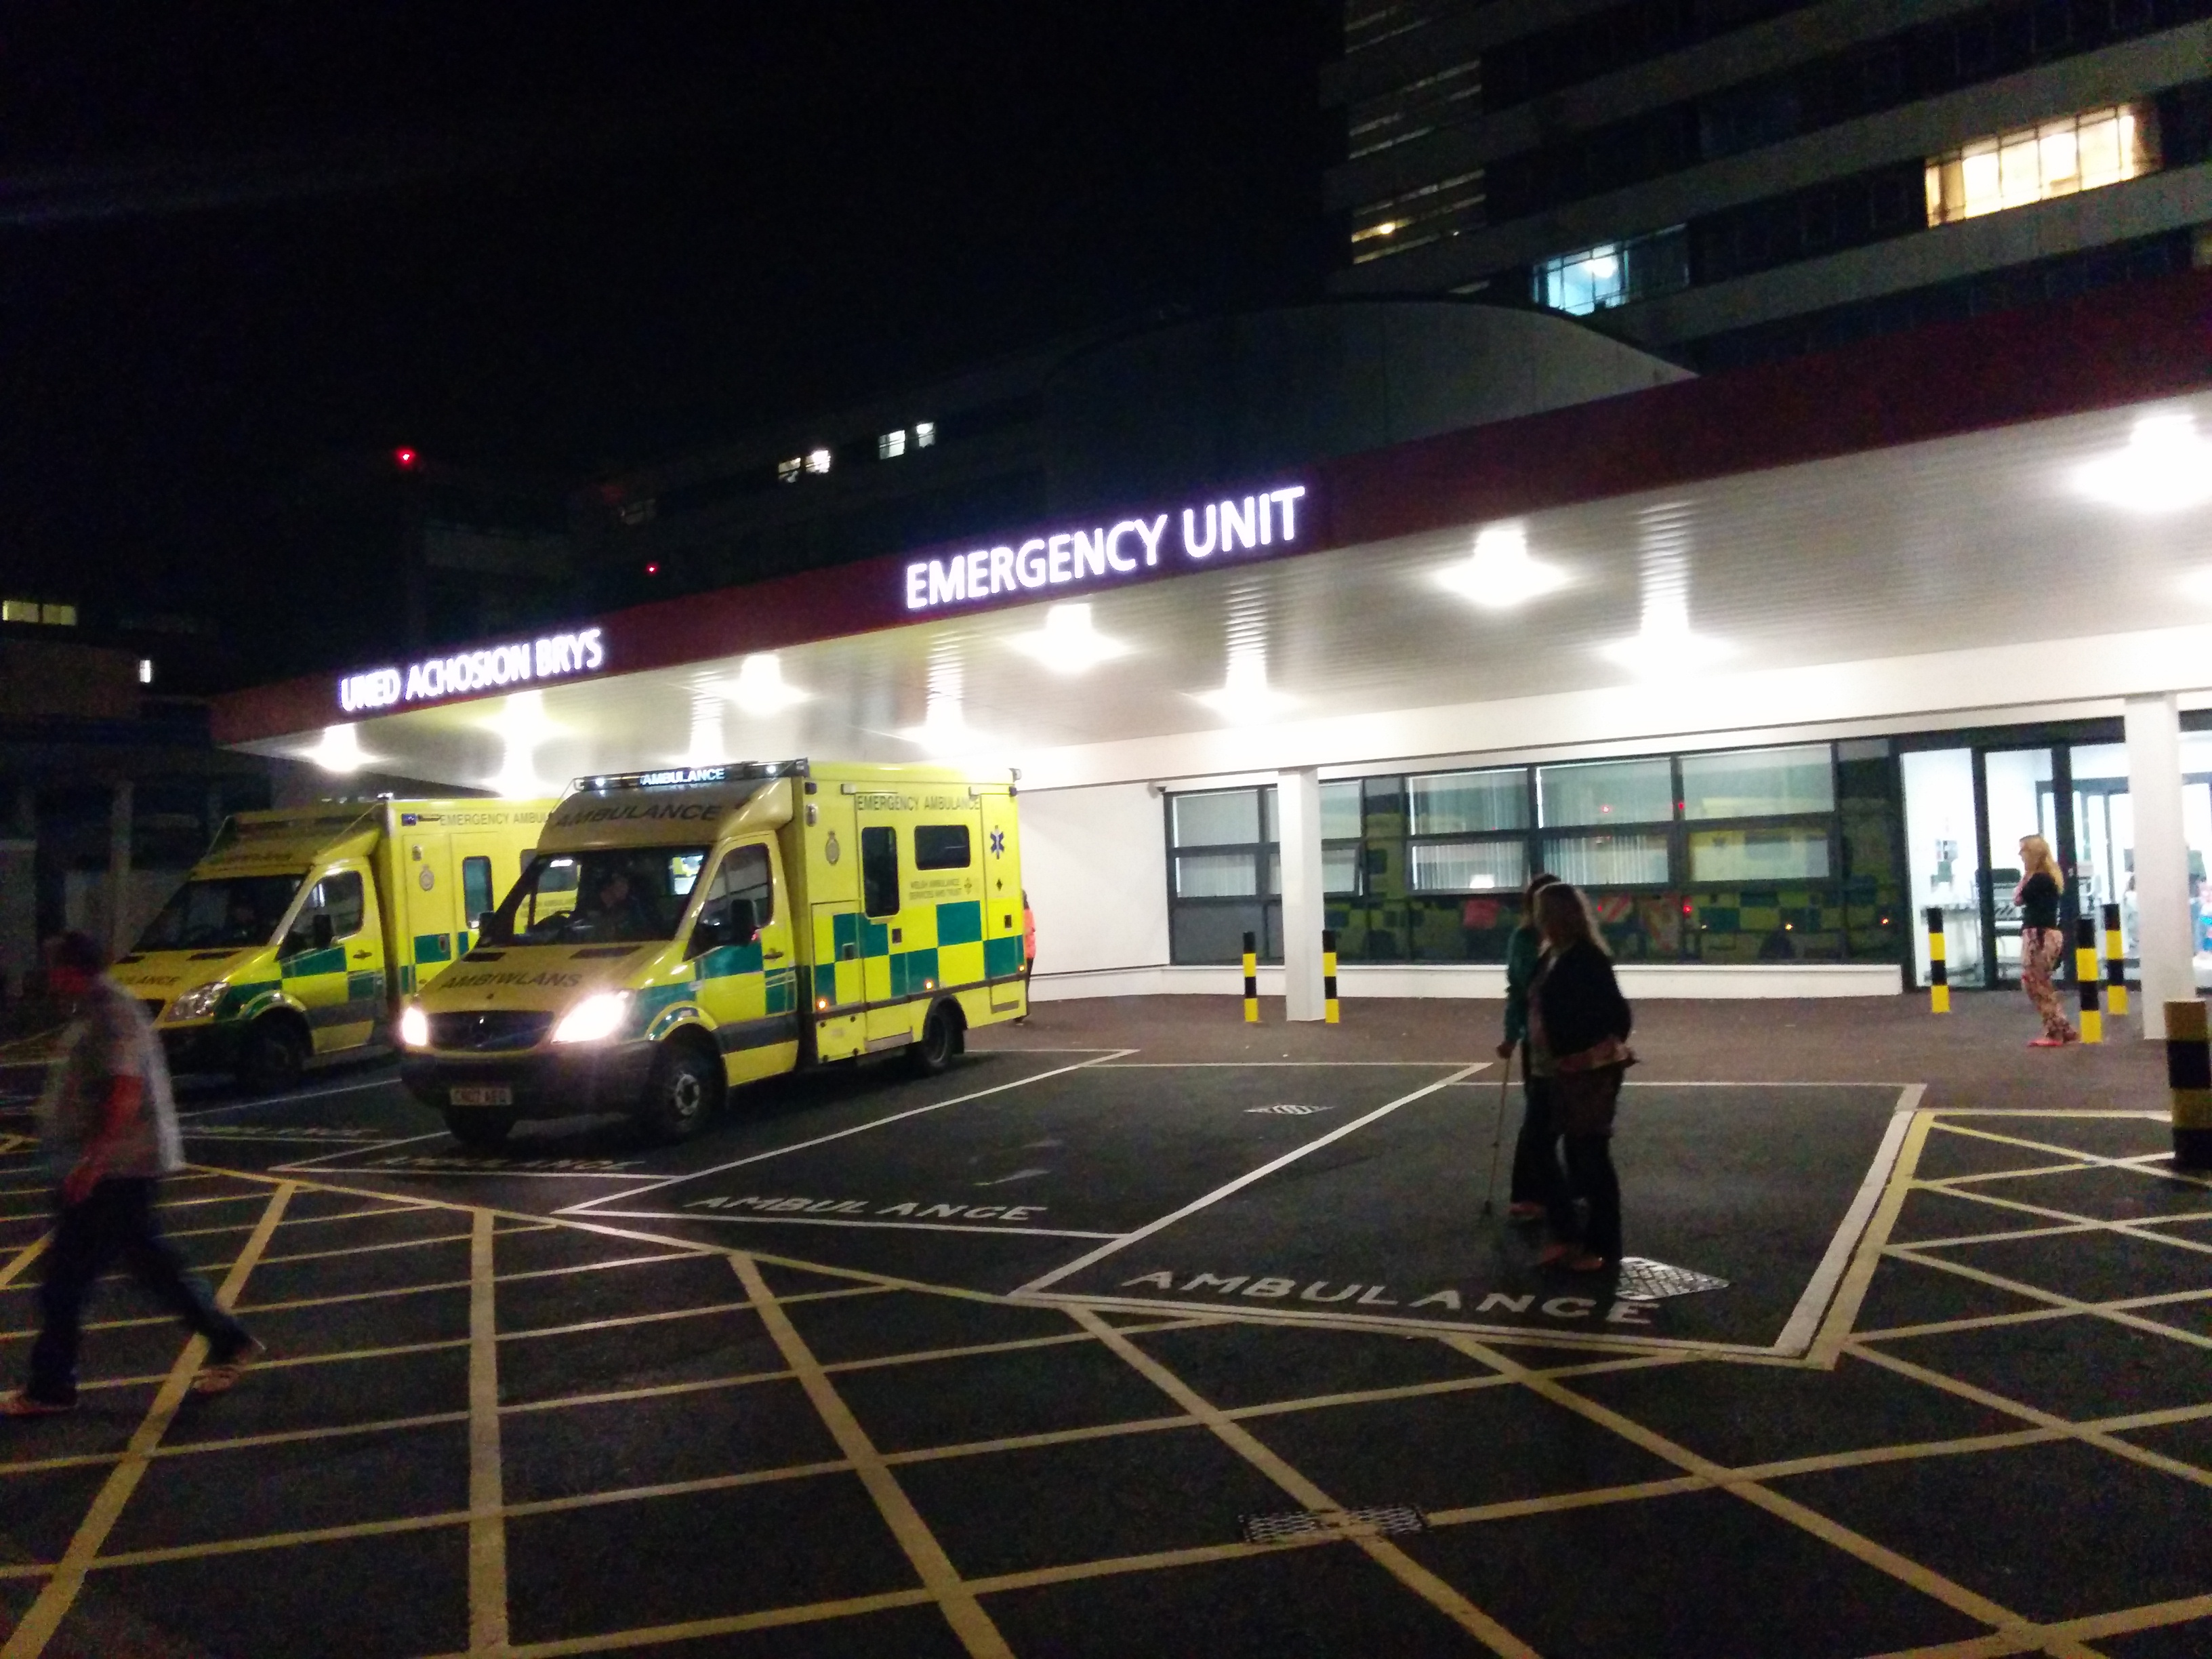
\includegraphics[width=.9\textwidth]{./Images/photo.jpg}
    \end{center}
}

\frame{
    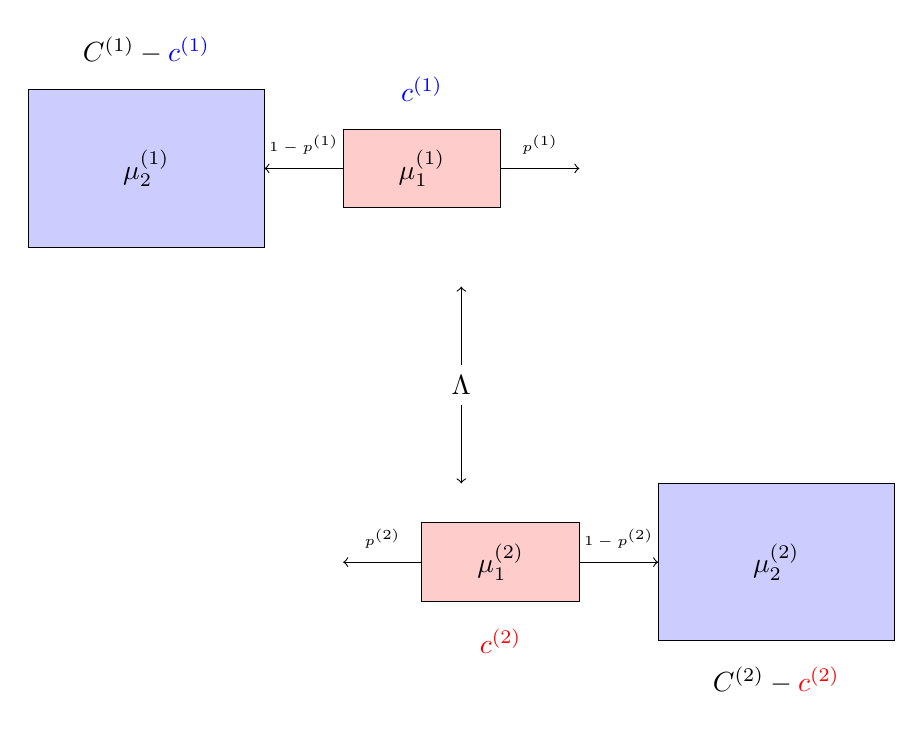
\begin{tikzpicture}
        % First hospital
        \draw [fill=blue!20] (0,0) rectangle (3,2);
        \draw [fill=red!20] (4,.5) rectangle (6,1.5);
        \draw [<-] (3,1) -- (4,1);
        \draw [<-] (7,1) -- (6,1);
        \node at (3.5, 1.3) {\tiny{$1-p^{(1)}$}};
        \node at (6.5, 1.3) {\tiny{$p^{(1)}$}};
        \node at (1.5,2.5) {$C^{(1)} - \color{blue}{c^{(1)}}$};
        \node at (5,2) {\color{blue}{$c^{(1)}$}};
        \node at (1.5,1) {$\mu_2^{(1)}$};
        \node at (5,1) {$\mu_1^{(1)}$};

        % Second hospital
        \draw [fill=red!20] (5,-3.5) rectangle (7,-4.5);
        \draw [fill=blue!20] (8,-3) rectangle (11,-5);
        \draw [<-] (8,-4) -- (7,-4);
        \draw [<-] (4,-4) -- (5,-4);
        \node at (7.5, -3.7) {\tiny{$1-p^{(2)}$}};
        \node at (4.5, -3.7) {\tiny{$p^{(2)}$}};
        \node at (6,-5) {$\color{red}{c^{(2)}}$};
        \node at (9.5,-5.5) {$C^{(2)} - \color{red}{c^{(2)}}$};
        \node at (6,-4) {$\mu_1^{(2)}$};
        \node at (9.5,-4) {$\mu_2^{(2)}$};

        % Ambulance
        \node at (5.5,-1.75) {$\Lambda$};
        \draw [->] (5.5,-1.5) -- (5.5,-.5);
        \draw [->] (5.5,-2) -- (5.5,-3);
    \end{tikzpicture}
}

\frame{
    \begin{center}
        \tikzstyle{level 1}=[level distance=3.5cm, sibling distance=3.5cm]
        \tikzstyle{level 2}=[level distance=3.5cm, sibling distance=2cm]
        \tikzstyle{player} = [text width=5em, draw, text centered, rectangle, fill=blue!20, inner sep=1pt]
        \tikzstyle{nature} = [minimum width=3pt,circle,  draw, fill=red!20, inner sep=1pt]
        \tikzstyle{end} = [circle, minimum width=3pt, fill, inner sep=0pt, right]
        \tikzstyle{corner} = [inner sep=0pt, outer sep=0pt, draw,circle]
        \begin{tikzpicture}[grow=right, sloped, scale=.6]
            \node[player]{Hospital 1}
            child {node [corner] (A1) {} node [right=2pt]{$C^{(1)} - 1$} }
            child {node [corner] (A2) {} node [right=2pt] {$1$} edge from parent node[above] {$\color{blue}{c^{(1)}}$}} ;
            \draw [bend right, dashed] (A1) to (A2);
            \node (B3) [player,right=3pt] at ($(A1)!0.5!(A2)$) {Hospital 2}
            child {node [corner] (A3) {} node [right=2pt]{$C^{(2)} - 1$} }
            child {node [corner] (A4) {} node [right=2pt] {$1$} edge from parent node[above] {$\color{red}{c^{(2)}}$}} ;
            \draw [bend right] (A3) to (A4);
            \node (e) [player,right=3pt] at ($(A3)!0.5!(A4)$) {Ambulance}
            child {node [corner] (A5) {} node [right=2pt]{$\Lambda$} }
            child {node [corner] (A6) {}  node [right=2pt] {$0$}edge from parent node[above] {$\lambda_1$}} ;
            \draw [bend right] (A5) to (A6);
            \node (e) [end,right=7pt] at ($(A5)!0.5!(A6)$) {};
        \end{tikzpicture}
    \end{center}
    \pause
    \vspace{1cm}
    $$(|u_1^{(1)}-u_2^{(1)}|,|u_1^{(2)}-u_2^{(2)}|,|w^{(1)}-w^{(2)}|)$$
}

\frame{
    $$
        S = \left\{(i,j)\in\mathbb{Z}^{2}_{\geq 0}\;|\;0\leq j \leq c_1+c_2,\; 0\leq i\leq c_1+N-\max(j-c_2,0)\right\}
    $$

    \centering
    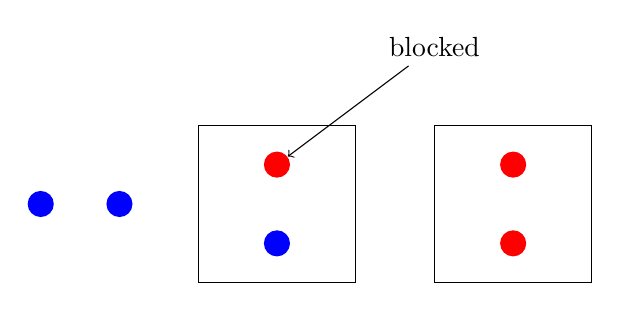
\begin{tikzpicture}
        \draw (0,1) rectangle (2,3);
        \draw (3,1) rectangle (5,3);

        \node at (1,1.5) [circle, fill, color=blue] {};
        \node (blocked) at (1,2.5) [circle, fill, color=red] {};

        \node at (-1,2) [circle, fill, color=blue] {};
        \node at (-2,2) [circle, fill, color=blue] {};

        \node at (4,1.5) [circle, fill, color=red] {};
        \node at (4,2.5) [circle, fill, color=red] {};

        \node (label) at (3,4) {blocked};
        \draw [->] (label) -- (blocked);
    \end{tikzpicture}
}

\frame{
    $$
    q_{(i_1,j_1), (i_2,j_2)}=
    \begin{cases}
        \Lambda, & \text{ if } \delta = (1,0)\\
        \min(c_1-\max(j_1-c_2,0),i_1)(1-p)\mu_1, & \text{ if } \delta = (-1,1)\\
        \min(c_1-\max(j_1-c_2,0),i_1)p\mu_1, & \text{ if } \delta = (-1,0)\\
        \min(c_2, j_1)\mu_2, & \text{ if } \delta = (0,-1)
    \end{cases}
    $$
}

\frame{
    \begin{center}
    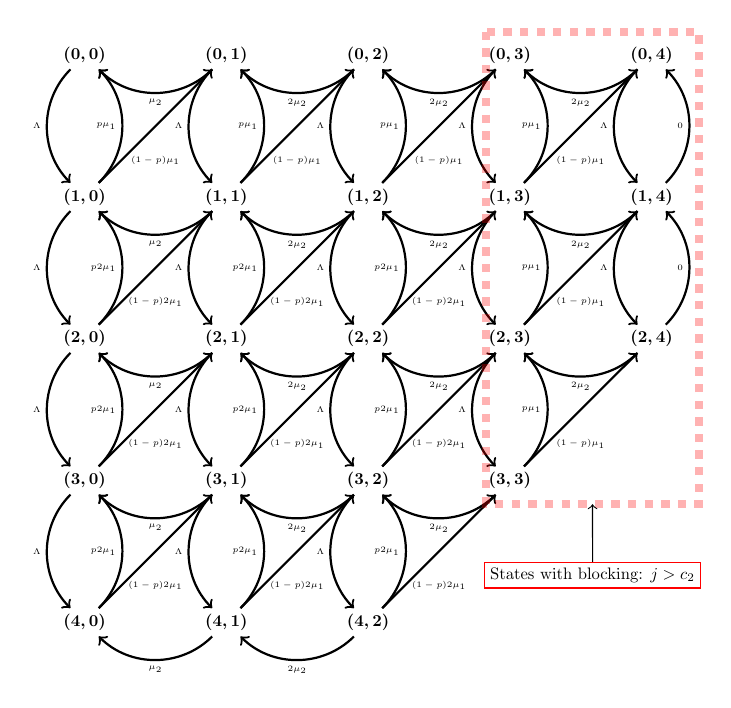
\begin{tikzpicture}[scale=.6, every node/.style={scale=0.6}]
    \tikzstyle{state}=[minimum width=2cm, font=\boldmath];
    % First row
    \node (00) at (0,0) [state] {$(0,0)$};
    \node (01) at ($(00)+(3,0)$) [state] {$(0,1)$};
    \node (02) at ($(01)+(3,0)$) [state] {$(0,2)$};
    \node (03) at ($(02)+(3,0)$) [state] {$(0,3)$};
    \node (04) at ($(03)+(3,0)$) [state] {$(0,4)$};

    % Second row
    \node (10) at ($(00)+(0,-3)$) [state] {$(1,0)$};
    \node (11) at ($(10)+(3,0)$) [state] {$(1,1)$};
    \node (12) at ($(11)+(3,0)$) [state] {$(1,2)$};
    \node (13) at ($(12)+(3,0)$) [state] {$(1,3)$};
    \node (14) at ($(13)+(3,0)$) [state] {$(1,4)$};

    % Third row
    \node (20) at ($(10)+(0,-3)$) [state] {$(2,0)$};
    \node (21) at ($(20)+(3,0)$) [state] {$(2,1)$};
    \node (22) at ($(21)+(3,0)$) [state] {$(2,2)$};
    \node (23) at ($(22)+(3,0)$) [state] {$(2,3)$};
    \node (24) at ($(23)+(3,0)$) [state] {$(2,4)$};

    % Fourth row
    \node (30) at ($(20)+(0,-3)$) [state] {$(3,0)$};
    \node (31) at ($(30)+(3,0)$) [state] {$(3,1)$};
    \node (32) at ($(31)+(3,0)$) [state] {$(3,2)$};
    \node (33) at ($(32)+(3,0)$) [state] {$(3,3)$};

    % Fifth row
    \node (40) at ($(30)+(0,-3)$) [state] {$(4,0)$};
    \node (41) at ($(40)+(3,0)$) [state] {$(4,1)$};
    \node (42) at ($(41)+(3,0)$) [state] {$(4,2)$};

    % Transitions
    % Arrivals
    \draw (00) edge[out=-135,in=135,->,thick] node [left] {\tiny$\Lambda$} (10);
    \draw (01) edge[out=-135,in=135,->,thick] node [left] {\tiny$\Lambda$} (11);
    \draw (02) edge[out=-135,in=135,->,thick] node [left] {\tiny$\Lambda$} (12);
    \draw (03) edge[out=-135,in=135,->,thick] node [left] {\tiny$\Lambda$} (13);
    \draw (04) edge[out=-135,in=135,->,thick] node [left] {\tiny$\Lambda$} (14);

    \draw (10) edge[out=-135,in=135,->,thick] node [left] {\tiny$\Lambda$} (20);
    \draw (11) edge[out=-135,in=135,->,thick] node [left] {\tiny$\Lambda$} (21);
    \draw (12) edge[out=-135,in=135,->,thick] node [left] {\tiny$\Lambda$} (22);
    \draw (13) edge[out=-135,in=135,->,thick] node [left] {\tiny$\Lambda$} (23);
    \draw (14) edge[out=-135,in=135,->,thick] node [left] {\tiny$\Lambda$} (24);

    \draw (20) edge[out=-135,in=135,->,thick] node [left] {\tiny$\Lambda$} (30);
    \draw (21) edge[out=-135,in=135,->,thick] node [left] {\tiny$\Lambda$} (31);
    \draw (22) edge[out=-135,in=135,->,thick] node [left] {\tiny$\Lambda$} (32);
    \draw (23) edge[out=-135,in=135,->,thick] node [left] {\tiny$\Lambda$} (33);

    \draw (30) edge[out=-135,in=135,->,thick] node [left] {\tiny$\Lambda$} (40);
    \draw (31) edge[out=-135,in=135,->,thick] node [left] {\tiny$\Lambda$} (41);
    \draw (32) edge[out=-135,in=135,->,thick] node [left] {\tiny$\Lambda$} (42);

    % First Station Service and exit
    \draw (00) edge[out=-45,in=45,<-,thick] node [left] {\tiny$p\mu_1$} (10);
    \draw (01) edge[out=-45,in=45,<-,thick] node [left] {\tiny$p\mu_1$} (11);
    \draw (02) edge[out=-45,in=45,<-,thick] node [left] {\tiny$p\mu_1$} (12);
    \draw (03) edge[out=-45,in=45,<-,thick] node [left] {\tiny$p\mu_1$} (13);
    \draw (04) edge[out=-45,in=45,<-,thick] node [left] {\tiny$0$} (14);

    \draw (10) edge[out=-45,in=45,<-,thick] node [left] {\tiny$p2\mu_1$} (20);
    \draw (11) edge[out=-45,in=45,<-,thick] node [left] {\tiny$p2\mu_1$} (21);
    \draw (12) edge[out=-45,in=45,<-,thick] node [left] {\tiny$p2\mu_1$} (22);
    \draw (13) edge[out=-45,in=45,<-,thick] node [left] {\tiny$p\mu_1$} (23);
    \draw (14) edge[out=-45,in=45,<-,thick] node [left] {\tiny$0$} (24);

    \draw (20) edge[out=-45,in=45,<-,thick] node [left] {\tiny$p2\mu_1$} (30);
    \draw (21) edge[out=-45,in=45,<-,thick] node [left] {\tiny$p2\mu_1$} (31);
    \draw (22) edge[out=-45,in=45,<-,thick] node [left] {\tiny$p2\mu_1$} (32);
    \draw (23) edge[out=-45,in=45,<-,thick] node [left] {\tiny$p\mu_1$} (33);

    \draw (30) edge[out=-45,in=45,<-,thick] node [left] {\tiny$p2\mu_1$} (40);
    \draw (31) edge[out=-45,in=45,<-,thick] node [left] {\tiny$p2\mu_1$} (41);
    \draw (32) edge[out=-45,in=45,<-,thick] node [left] {\tiny$p2\mu_1$} (42);

    % First Station Service and ward
    \draw (01) edge[out=-135,in=45,<-,thick] node [right, below=.5cm] {\tiny$(1-p)\mu_1$} (10);
    \draw (02) edge[out=-135,in=45,<-,thick] node [right, below=.5cm] {\tiny$(1-p)\mu_1$} (11);
    \draw (03) edge[out=-135,in=45,<-,thick] node [right, below=.5cm] {\tiny$(1-p)\mu_1$} (12);
    \draw (04) edge[out=-135,in=45,<-,thick] node [right, below=.5cm] {\tiny$(1-p)\mu_1$} (13);

    \draw (11) edge[out=-135,in=45,<-,thick] node [right, below=.5cm] {\tiny$(1-p)2\mu_1$} (20);
    \draw (12) edge[out=-135,in=45,<-,thick] node [right, below=.5cm] {\tiny$(1-p)2\mu_1$} (21);
    \draw (13) edge[out=-135,in=45,<-,thick] node [right, below=.5cm] {\tiny$(1-p)2\mu_1$} (22);
    \draw (14) edge[out=-135,in=45,<-,thick] node [right, below=.5cm] {\tiny$(1-p)\mu_1$} (23);

    \draw (21) edge[out=-135,in=45,<-,thick] node [right, below=.5cm] {\tiny$(1-p)2\mu_1$} (30);
    \draw (22) edge[out=-135,in=45,<-,thick] node [right, below=.5cm] {\tiny$(1-p)2\mu_1$} (31);
    \draw (23) edge[out=-135,in=45,<-,thick] node [right, below=.5cm] {\tiny$(1-p)2\mu_1$} (32);
    \draw (24) edge[out=-135,in=45,<-,thick] node [right, below=.5cm] {\tiny$(1-p)\mu_1$}  (33);

    \draw (31) edge[out=-135,in=45,<-,thick] node [right, below=.5cm] {\tiny$(1-p)2\mu_1$} (40);
    \draw (32) edge[out=-135,in=45,<-,thick] node [right, below=.5cm] {\tiny$(1-p)2\mu_1$} (41);
    \draw (33) edge[out=-135,in=45,<-,thick] node [right, below=.5cm] {\tiny$(1-p)2\mu_1$} (42);

    % Second station services
    \draw (01) edge[out=-135,in=-45,->,thick] node [below] {\tiny$\mu_2$} (00);
    \draw (02) edge[out=-135,in=-45,->,thick] node [below] {\tiny$2\mu_2$} (01);
    \draw (03) edge[out=-135,in=-45,->,thick] node [below] {\tiny$2\mu_2$} (02);
    \draw (04) edge[out=-135,in=-45,->,thick] node [below] {\tiny$2\mu_2$} (03);

    \draw (11) edge[out=-135,in=-45,->,thick] node [below] {\tiny$\mu_2$}  (10);
    \draw (12) edge[out=-135,in=-45,->,thick] node [below] {\tiny$2\mu_2$} (11);
    \draw (13) edge[out=-135,in=-45,->,thick] node [below] {\tiny$2\mu_2$} (12);
    \draw (14) edge[out=-135,in=-45,->,thick] node [below] {\tiny$2\mu_2$} (13);

    \draw (21) edge[out=-135,in=-45,->,thick] node [below] {\tiny$\mu_2$}  (20);
    \draw (22) edge[out=-135,in=-45,->,thick] node [below] {\tiny$2\mu_2$} (21);
    \draw (23) edge[out=-135,in=-45,->,thick] node [below] {\tiny$2\mu_2$} (22);
    \draw (24) edge[out=-135,in=-45,->,thick] node [below] {\tiny$2\mu_2$} (23);

    \draw (31) edge[out=-135,in=-45,->,thick] node [below] {\tiny$\mu_2$}  (30);
    \draw (32) edge[out=-135,in=-45,->,thick] node [below] {\tiny$2\mu_2$} (31);
    \draw (33) edge[out=-135,in=-45,->,thick] node [below] {\tiny$2\mu_2$} (32);

    \draw (41) edge[out=-135,in=-45,->,thick] node [below] {\tiny$\mu_2$}  (40);
    \draw (42) edge[out=-135,in=-45,->,thick] node [below] {\tiny$2\mu_2$} (41);

    % Indicating phases corresponding to blockages
    \draw [dashed, line width=1mm, red, opacity=.3] ($(03) + (-.5,.5)$) rectangle ($(33) + (4,-.5)$);
    \node (label) at ($(33) + (1.75,-2)$) [draw=red] {States with blocking: $j>c_2$};
    \draw [->] (label) -- ($(33) + (1.75,-.5)$);

\end{tikzpicture}

    \end{center}
}

\frame{

    \begin{columns}
        \column{.5\textwidth}
        \begin{center}
        \texttt{Analytical}
        \includegraphics[width=\textwidth]{./Images/{10.000-15.000-12.000-4.000-0.400-1.000-0.200-40000.000-10000.000-32-markov_chain}.pdf}\\
        \includegraphics[width=\textwidth]{./Images/{10.000-15.000-12.000-5.000-0.400-1.000-0.200-40000.000-10000.000-32-markov_chain}.pdf}
        \end{center}
        \column{.5\textwidth}
        \begin{center}
        \texttt{Simulation}
        \includegraphics[width=\textwidth]{./Images/{10.000-15.000-12.000-4.000-0.400-1.000-0.200-40000.000-10000.000-32-simulation}.pdf}\\
        \includegraphics[width=\textwidth]{./Images/{10.000-15.000-12.000-5.000-0.400-1.000-0.200-40000.000-10000.000-32-simulation}.pdf}
        \end{center}
    \end{columns}
}

\frame{
    Expected wait:
    $$
    w = \frac{\sum_{(i,j)\in S_A}c(i,j)\pi_{(i,j)}}{\sum_{(i,j)\in S_A}\pi_{(i,j)}}
    $$
    \begin{center}
        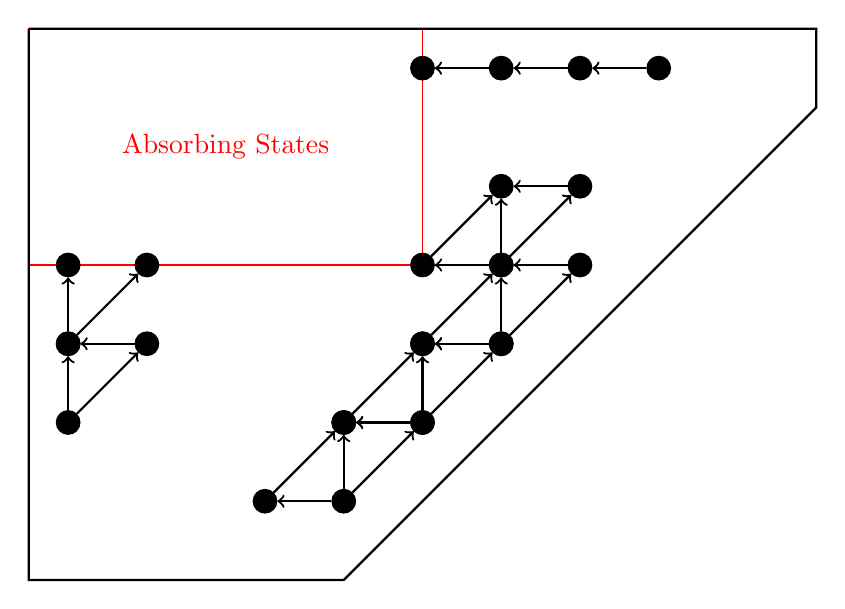
\begin{tikzpicture}
            \tikzstyle{vertex} = [draw, shape=circle, minimum width=.3cm, inner sep=.5pt, fill=black]
            \draw [red] (0,0) rectangle (5,-3);
            \draw [thick](0,0) -- (10,0) -- (10,-1) -- (4,-7) -- (0,-7) -- (0,0);
            \node at (2.5,-1.5) [red] {Absorbing States};

            \node (1) [vertex] at (4,-6) {};
            \node (2) [vertex] at ($(1)+(1,1)$) {};
            \node (3) [vertex] at ($(1)+(0,1)$) {};
            \node (4) [vertex] at ($(1)+(-1,0)$) {};
            \draw (1) edge[->, thick] (2);
            \draw (1) edge[->, thick] (3);
            \draw (1) edge[->, thick] (4);
            \draw (2) edge[->, thick] (3);
            \draw (4) edge[->, thick] (3);

            \node (1) [vertex] at (2) {};
            \node (2) [vertex] at ($(1)+(1,1)$) {};
            \node (3) [vertex] at ($(1)+(0,1)$) {};
            \node (4) [vertex] at ($(1)+(-1,0)$) {};
            \draw (1) edge[->, thick] (2);
            \draw (1) edge[->, thick] (3);
            \draw (1) edge[->, thick] (4);
            \draw (2) edge[->, thick] (3);
            \draw (4) edge[->, thick] (3);

            \node (1) [vertex] at (2) {};
            \node (2) [vertex] at ($(1)+(1,1)$) {};
            \node (3) [vertex] at ($(1)+(0,1)$) {};
            \node (4) [vertex] at ($(1)+(-1,0)$) {};
            \draw (1) edge[->, thick] (2);
            \draw (1) edge[->, thick] (3);
            \draw (1) edge[->, thick] (4);
            \draw (2) edge[->, thick] (3);
            \draw (4) edge[->, thick] (3);

            \node (1) [vertex] at (3) {};
            \node (2) [vertex] at ($(1)+(1,1)$) {};
            \node (3) [vertex] at ($(1)+(0,1)$) {};
            \node (4) [vertex] at ($(1)+(-1,0)$) {};
            \draw (1) edge[->, thick] (2);
            \draw (1) edge[->, thick] (3);
            \draw (1) edge[->, thick] (4);
            \draw (2) edge[->, thick] (3);
            \draw (4) edge[->, thick] (3);

            \node (1) [vertex] at (.5,-5) {};
            \node (2) [vertex] at ($(1)+(0,1)$) {};
            \node (3) [vertex] at ($(1)+(1,1)$) {};
            \draw (1) edge[->, thick] (2);
            \draw (1) edge[->, thick] (3);
            \draw (3) edge[->, thick] (2);

            \node (1) [vertex] at (2) {};
            \node (2) [vertex] at ($(1)+(0,1)$) {};
            \node (3) [vertex] at ($(1)+(1,1)$) {};
            \draw (1) edge[->, thick] (2);
            \draw (1) edge[->, thick] (3);

            \node (1) [vertex] at (8,-.5) {};
            \node (2) [vertex] at ($(1)+(-1,0)$) {};
            \node (3) [vertex] at ($(2)+(-1,0)$) {};
            \node (4) [vertex] at ($(3)+(-1,0)$) {};

            \draw (1) edge[->, thick] (2);
            \draw (2) edge[->, thick] (3);
            \draw (3) edge[->, thick] (4);
        \end{tikzpicture}
    \end{center}
    }

\frame{
    Sojourn time in state $(i,j)$:
    $$
    w(i,j)=\frac{1}{\min(c_2,j)\mu_2+\min(c_1-\max(j-c_2,0),i)\mu_1}
    $$

    Cost of state $(i,j)$:
    $$
    \tiny{
        c(i,j) = \begin{cases}
            0,&\text{ if }(i,j)\in A\\
            w(i,j) + p_{s_2}c(i,j-1)+p_{s_1}(pc(i-1,j)+(1-p)c(i-1,j+1)), &\text{ otherwise}
        \end{cases}
    }
    $$
    \begin{center}
        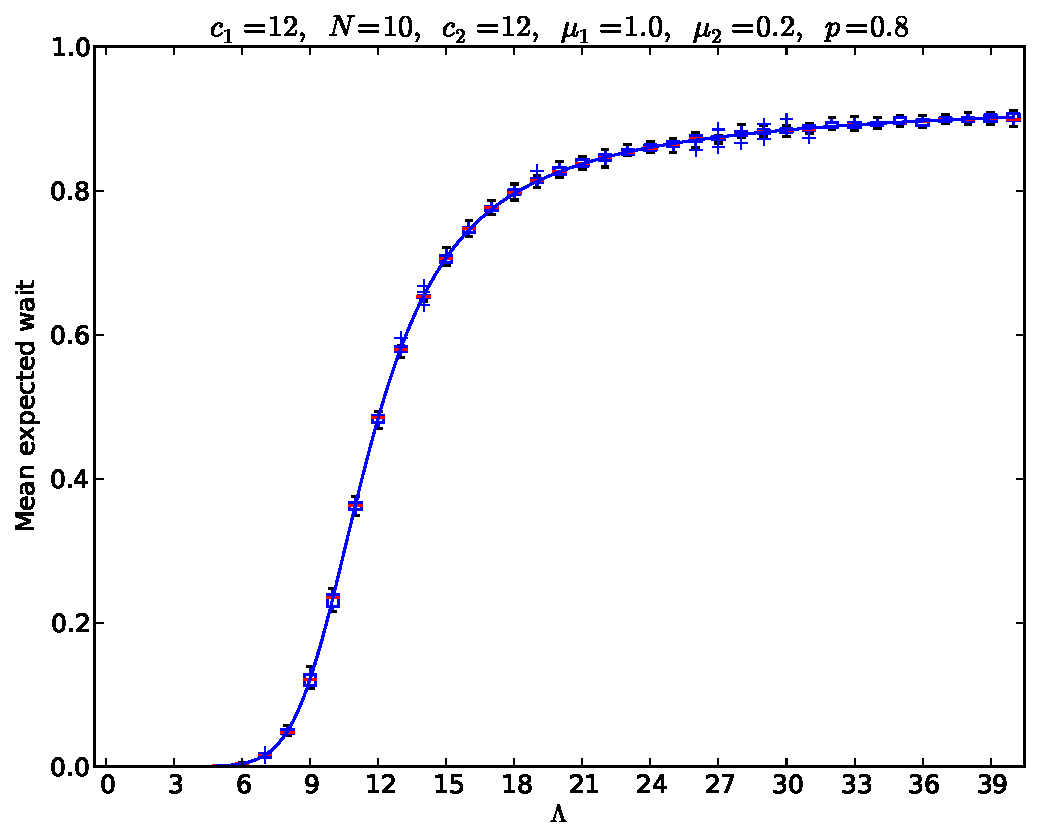
\includegraphics[width=.6\textwidth]{./Images/12-10-12-1.0-0.2-0.8.pdf}
    \end{center}

}

\frame{
    $$
    f(\lambda)=w^{(1)}(\lambda)-w^{(2)}(\Lambda-\lambda)
    $$

    \begin{center}
        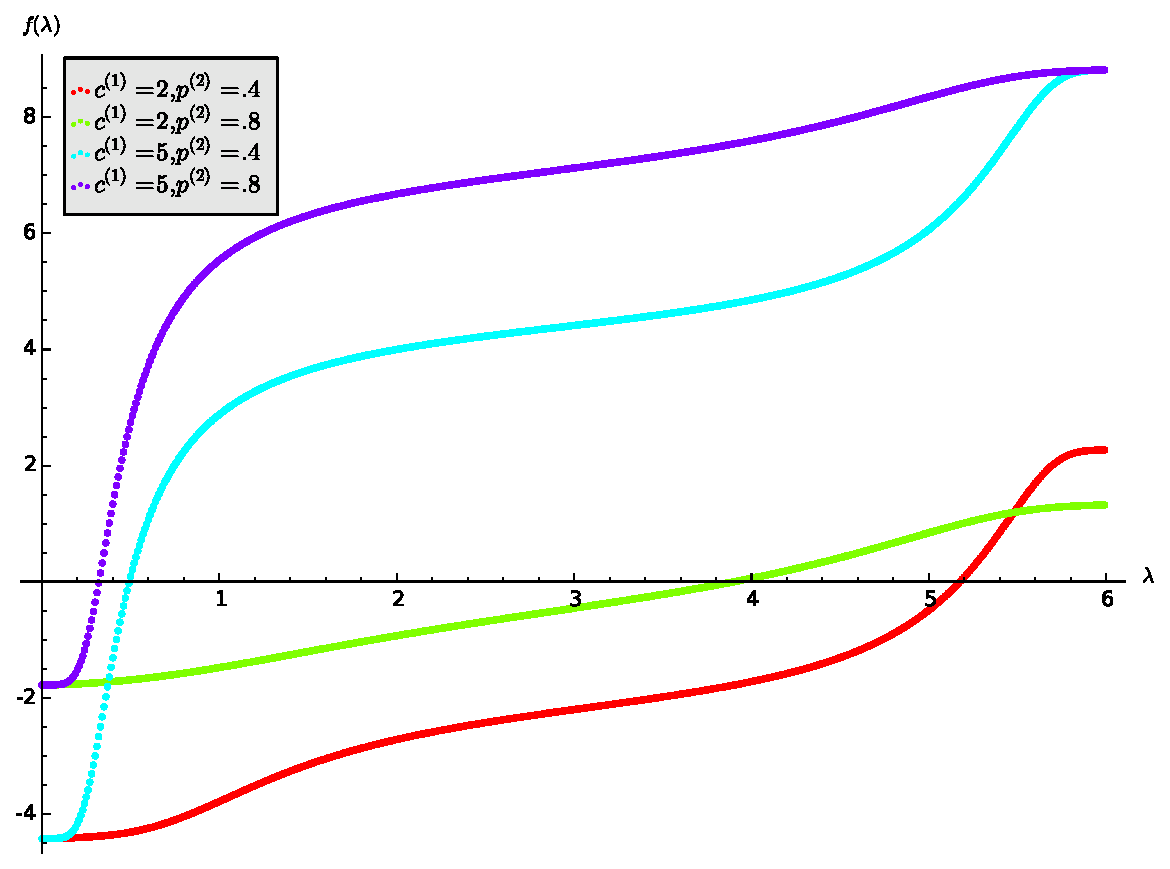
\includegraphics[width=.9\textwidth]{./Images/plot-of-f.pdf}
    \end{center}
}

\frame{
    \begin{center}
        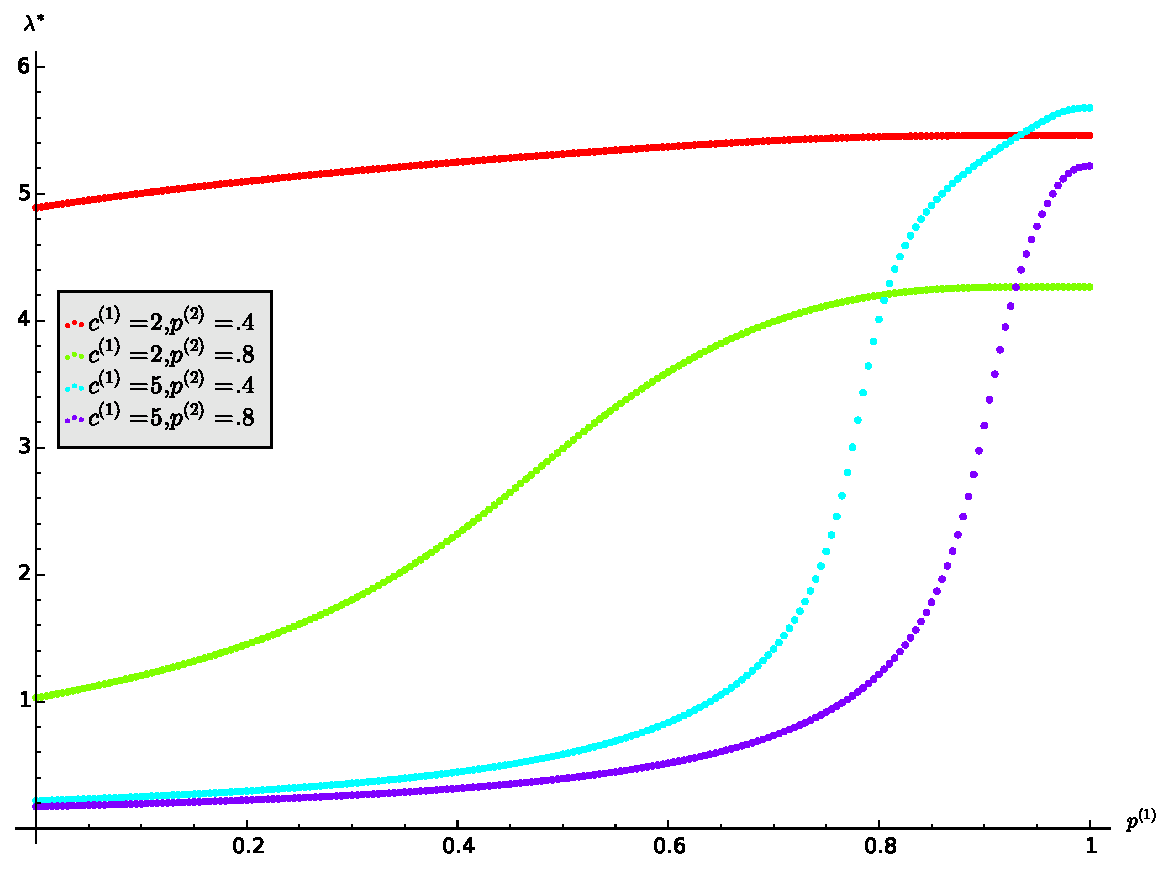
\includegraphics[width=\textwidth]{./Images/plot-lambda-star.pdf}
    \end{center}
}

\frame{
    $$\Lambda=6, C^{(1)}=6, C^{(2)}=4, N^{(1)}=N^{(2)}=3$$
    $$
    A=
    \left(\begin{array}{rrr}
        0.795 & 0.688 & 0.792 \\
        0.506 & 0.488 & 0.503 \\
        0.183 & 0.159 & 0.178 \\
        0.0104 & 0.0193 & 0.00523 \\
        0.0121 & 0.108 & 0.0159
    \end{array}\right)
    B=
    \left(\begin{array}{rrr}
        0.667 & 0.243 & 0.00105 \\
        0.480 & 0.154 & 0.196 \\
        0.396 & 0.0774 & 0.253 \\
        0.470 & 0.140 & 0.205 \\
        0.664 & 0.239 & 0.00837
    \end{array}\right)
    $$
    $$
    \lambda_1=
    \left(\begin{array}{rrr}
        3.17 & 1.18 & 2.88 \\
        5.18 & 3.90 & 4.87 \\
        5.37 & 4.39 & 5.07 \\
        5.21 & 4.01 & 4.90 \\
        3.46 & 1.67 & 3.18
    \end{array}\right)
    S=
    \left(\begin{array}{rrr}
        0.672 & 0.481 & 0.672 \\
        0.381 & 0.427 & 0.429 \\
        0.315 & 0.341 & 0.352 \\
        0.376 & 0.418 & 0.423 \\
        0.666 & 0.535 & 0.671
    \end{array}\right)
    $$
    \pause
    \begin{center}
        $\tilde c_1=4, \tilde c_2=2$ and $c_1^*=3, c_2^*=1$ for $\text{PoA}=1.330$.
    \end{center}
}

\frame{
    \begin{center}
        \begin{tikzpicture}
            \node at (0,0) {$\displaystyle{\text{PoA}=\frac{\tilde c_1 S \tilde c_2}{c_1^* S c_2 ^*}=\frac{\tilde c_1 S \tilde c_2}{\min S}}$};
            \node at (3.5,-3) {};
            \pause
            \node (a) at (0,2) {from $A,B$};
            \draw (a) edge[out=180, in=135, ->, color=red] (-.75,.5);
            \draw (a) edge[out=0, in=45, ->, color=red] (.25,.5);
            \pause
            \node (b) at (-1,-2) {from $f(\lambda)$};
            \draw (b) edge[out=180, in=135, ->, color=blue] (a);
        \end{tikzpicture}
    \end{center}
}

\frame{
Effect of p1
}

\frame{
Effect of lambda
}

\frame{
Effect of C
}

\frame{
\begin{center}
\href{https://plus.google.com/+VincentKnight/posts}{+Vincent.Knight}\\
\href{https://twitter.com/drvinceknight}{@drvinceknight}\\
\href{http://drvinceknight.github.io/Talks/}{vincent-knight.com/Talks}\\
\end{center}
}

\end{document}
